\immediate\write18{makeindex \jobname.nlo -s nomencl.ist -o
\jobname.nls }
 \documentclass[12pt]  {article}%{scrartcl}
 \topmargin=0.3in \textheight=8.6in \hoffset=-0.8in \textwidth=7in
 %  The Useful package I used
%%%%%%%%%%%%%%%%%%%%%%%%%%%%%%%%%%%%%%%%%%%%%%%%%%%%%%%%%%%%%%%%%%%%%
% The following packages help to define the default font and style
\usepackage{perpage} %the perpage package
\MakePerPage{footnote} %the perpage package command
% to fix the footnote does not show
%\protect\footnote{your note}
\usepackage{multicol}% for multi column
\usepackage{pdfpages} %using for adding PDF pages
\usepackage{helvet}
\usepackage[T1]{fontenc}
\usepackage[math]{anttor}
\usepackage[full]{textcomp}
\usepackage{libris}
%%%%%%%%%%%%%%%%%%%%%%%%%%%%%%%%%%%%%%%%%%%%%%%%%%%%%%%%%%%%%%%%%%%%%
\usepackage{color}
\usepackage{subfigure}
\usepackage[nottoc]{tocbibind}
\usepackage{amsthm}
\usepackage{psfrag,graphicx,amsmath,amssymb,amsfonts}
\usepackage{tikz}
\usetikzlibrary{patterns}
\usepackage{algorithm}
\usepackage{algpseudocode}
\usepackage{verbatim}
\usepackage{graphicx}
\usepackage{latexsym}
\usepackage{booktabs}
\usepackage{longtable}
\usepackage{multirow}
\usepackage{epsfig}
\usepackage{nomencl}   % To generate the Notation
\renewcommand{\nomname}{List of Notations}
\renewcommand*{\pagedeclaration}[1]{\unskip\dotfill\hyperpage{#1}}
\makenomenclature
 \usepackage{kpfonts} %[uprightRoman, uprightgreeks]
 \usepackage[T1]{fontenc}
 \usepackage[colorlinks=true,linkcolor=blue,citecolor=blue,urlcolor=blue,pagebackref]{hyperref}
% \hypersetup{linkcolor = black}
%\listoffigures
%\hypersetup{linkcolor = red}
 \usepackage[subfigure]{tocloft}
   \setlength\cftbeforefigskip{1 ex} % list of figures
   \setlength\cftbeforetabskip{1 ex} % list of tables
   \setlength\cftbeforesecskip{1 em} % spacing before sec title
   \setlength\cftaftertoctitleskip{1.8 em}
   \setlength\cftbeforetoctitleskip{4 cm}
   \setlength{\nomitemsep}{0.5 ex}
 \usepackage{titlesec}
 %\titleformat{\subsection} {\large \bfseries \color{blue}} {\thesubsection}{1 ex}{}
 %\titleformat{\subsubsection}  {\normalsize  \bfseries  \color{blue}}       {\thesubsubsection}{1 ex}{}  %\slshape
 \setcounter{tocdepth}{3}   % table of content depth
\definecolor{RoyalBlue}{RGB}{0, 35, 102}
\usepackage{lineno}  % To add the line number
\setpagewiselinenumbers
\modulolinenumbers[1]
%%%%%%%%%%%%%%%%%%%%%%%%%%%%%%%%%%%%%%%%%%%%%%%%%%%%%%%%%%%%
\usepackage{listings}  % Source Code display style

\lstdefinestyle{customc}{
  belowcaptionskip=1\baselineskip,
  breaklines=true,
  frame=single,%single,L
  xleftmargin=\parindent,
  language=C,
  showstringspaces=false,
  basicstyle=\footnotesize\ttfamily,
  keywordstyle=\bfseries\color{blue!40!black},
  commentstyle=\itshape\color{purple!40!black},
  identifierstyle=\color{blue},
  stringstyle=\color{orange},
}

\lstdefinestyle{customasm}{
  belowcaptionskip=1\baselineskip,
  frame=L,
  xleftmargin=\parindent,
  language=[x86masm]Assembler,
  basicstyle=\footnotesize\ttfamily,
  commentstyle=\itshape\color{purple!40!black},
}
\lstset{escapechar=@,style=customc}


%%%%%%%%%%%%%%The Appendix%%%%%%%%%%%%%%%%%%%%%%%%%%
%\usepackage[title,titletoc,toc]{appendix}
\renewcommand{\appendix}{\newpage
  \setcounter{section}{0}
  \setcounter{subsection}{0}
  \setcounter{figure}{0}
  \setcounter{table}{0}
  \addcontentsline{toc}{section}{Appendices}
  \section*{Appendices}
  \renewcommand\thesection{\Alph{section}}
  \renewcommand\thefigure{\Alph{section}\arabic{figure}}
  \renewcommand\thetable{\Alph{section}\arabic{table}}
}

%\newcommand{\startappendix}{%
%\pagebreak%
%\addcontentsline{toc}{section}{Appendices}%
%%\fancyhead[L]{{\bfseries Appendices}}%
%\setcounter{section}{0}%
%\renewcommand{\thesection}{\Alph{section}}%
%}
%
%\newenvironment{newappendix}[2]%
%{\gdef\headername{#1}%
%\phantomsection%
%\refstepcounter{section}%
%\addcontentsline{toc}{section}{Appendix \thesection~- #1}%
%\label{app:#2}}
%{\fancyhead[R]{Appendix \thesection~- \headername}
%\newpage}
%
%%%%%%%%%%%The headers and footers %%%%%%%%%%%%%%%
\usepackage{lastpage}
\usepackage{fancyhdr}
\pagestyle{fancy}
\lhead{Wenqiang Feng}
\chead{Prelim Exam note  for Numerical Analysis}
\rhead{Page \thepage}
\cfoot{ Page\ \thepage\ of\ \protect\pageref{LastPage}}
\renewcommand{\headrulewidth}{0.4pt}
\renewcommand{\footrulewidth}{0.4pt}

 %multigrid{\cal F}
\newcommand{\calFc}{\mathcal{F}_c}
\newcommand{\calFe}{\mathcal{F}_e}
\newcommand{\Rh}{\mathcal{R}_h}
\newcommand{\Bisel}{\mathcal{B}_\ell}
\newcommand{\Biselml}{\mathcal{B}_{\ell-1}}
\newcommand{\Rsel}{\mathcal{R}_\ell}
\newcommand{\pRselml}{\mathcal{R}_{\ell-1}}
\newcommand{\pRj}{\mathcal{R}_{j}}
\newcommand{\bil}[1]{a\left (#1\right)}
\newcommand{\diam}{\operatorname{diam}}
\newcommand{\MG}[1]{\textsc{MG}\left(#1\right)}
\newcommand{\TGsl}[1]{\textsc{TG}_1\left(#1\right)}
\newcommand{\TGsel}[1]{\textsc{TG}_\ell\left(#1\right)}
\newcommand{\Mn}{\mathcal{M}_{n}}
\newcommand{\Mnn}{\mathcal{M}_{n\times n}}
\newcommand{\Mmn}{\mathcal{M}_{m\times n}}
\newcommand{\vomega}{\vec{\omega}}
\newcommand{\vomegaseln}{\vec{\omega}_\ell}
\newcommand{\vomegasel}[1]{\vec{\omega}_\ell^{(#1)}}
\newcommand{\epislonsel}[1]{{\epsilon}_\ell^{(#1)}}
\newcommand{\vomegaselsk}{\vec{\omega}~_\ell^{(k)}}
\newcommand{\vomegaselml}{\vec{\omega}_{\ell-1}}
\newcommand{\omeso}{\omega_0}
\newcommand{\epssk}{\epsilon_k}
\newcommand{\epssnk}{\epsilon_{n_1+1-k}}
\newcommand{\alphask}{\alpha_k}
\newcommand{\alphasno}{\alpha_{n_0+1}}
\newcommand{\betask}{\beta_k}
\newcommand{\etaselsk}{\eta_\ell^{(k)}}
\newcommand{\betasno}{\beta_{n_0+1}}
\newcommand{\no}{n_0}
\newcommand{\nsel}{n_\ell}
\newcommand{\msel}{m_\ell}
\newcommand{\hsel}{h_\ell}
\newcommand{\hselml}{h_{\ell-1}}
\newcommand{\nselml}{n_{\ell-1}}
\newcommand{\rhosone}{\rho_1}
\newcommand{\rhosel}{\rho_\ell}
\newcommand{\Tso}{\mathcal{T}_0}
\newcommand{\Tsl}{\mathcal{T}_1}
\newcommand{\Tsel}{\mathcal{T}_\ell}
\newcommand{\Tselml}{\mathcal{T}_{\ell-1}}
\newcommand{\Vsel}{V_\ell}
\newcommand{\Hsel}{H_\ell}
\newcommand{\BselsV}{B_\ell^V}
\newcommand{\BselsW}{B_\ell^W}
\newcommand{\Wsel}{W_\ell}
\newcommand{\Vselml}{V_{\ell-1}}
\newcommand{\vselml}{v_{\ell-1}}
\newcommand{\vselmlsi}{v_{\ell-1,i}}
\newcommand{\vselsi}{v_{\ell,i}}
\newcommand{\vselsj}{v_{\ell,j}}
\newcommand{\vsel}{v_\ell}
\newcommand{\wsel}{w_\ell}
\newcommand{\vvselsnsel}{\vec{v}_\ell^{(n_\ell)}}
\newcommand{\vvselsl}{\vec{v}_\ell^{(1)}}
\newcommand{\vvselsp}{\vec{v}~_\ell^{'}}
\newcommand{\vvselstp}{\vec{v}~_\ell^{''}}
\newcommand{\Bsel}{B_\ell}
\newcommand{\Bselml}{B_{\ell-1}}
\newcommand{\TsL}{\mathcal{T}_L}
\newcommand{\Tsx}[1]{\mathcal{T}_{#1}}
\newcommand{\Io}{I_o}
\newcommand{\il}{I_1}
\newcommand{\Cl}{C_1}
\newcommand{\Laml}{\Lambda_1}
\newcommand{\lamselsl}{\lambda_\ell^{(1)}}
\newcommand{\lamselsnsel}{\lambda_\ell^{(\nsel)}}
\newcommand{\lamselsk}{\lambda_\ell^{(k)}}
\newcommand{\Lamsel}{\Lambda_\ell}
\newcommand{\Lamselsml}{\Lambda_\ell^{-1}}
\newcommand{\invLaml}{\Lambda_1^{-1}}
\newcommand{\ml}{m_1}
\newcommand{\mll}{m_2}
\newcommand{\nl}{n_1}
\newcommand{\Ao}{A_0}
\newcommand{\AL}{A_L}
\newcommand{\AsL}{A_L}
\newcommand{\Ah}{A_h}
\newcommand{\AH}{A_H}
\newcommand{\Al}{A_1}
\newcommand{\Ael}{A_\ell}
\newcommand{\Asel}{A_\ell}
\newcommand{\Msel}{M_\ell}
\newcommand{\Asj}{A_j}
\newcommand{\Aselml}{A_{\ell-1}}
\newcommand{\Relml}{R_{\ell-1}}
\newcommand{\Pselml}{P_{\ell-1}}
\newcommand{\Ro}{R_0}
\newcommand{\Rl}{R_1}
\newcommand{\Rel}{R_\ell}
\newcommand{\Rselml}{R_{\ell-1}}
\newcommand{\nelml}{n_{\ell-1}}
\newcommand{\Po}{P_0}
\newcommand{\Pl}{P_1}
\newcommand{\Psel}{P_\ell}
\newcommand{\QselsL}{Q_\ell^L}
\newcommand{\Pelml}{P_{\ell-1}}
%\newcommand{\Pselml}{P_{\ell-1}}
\newcommand{\vu}{\vec{u}}
\newcommand{\vz}{\vec{z}}
\newcommand{\vv}{\vec{v}}
\newcommand{\vvkl}{\vec{v}~^{k+1}}
\newcommand{\vx}{\vec{x}}
\newcommand{\vuk}{\vec{u}~^k}
\newcommand{\vukhalf}{\vec{u}~^{k+1/2}}
\newcommand{\vuo}{\vec{u}~^0}
\newcommand{\uo}{u_0}
\newcommand{\ul}{u_1}
\newcommand{\vo}{\vec{0}}
\newcommand{\vul}{\vec{u}~^1}
\newcommand{\usel}{\vec{u}_\ell}
\newcommand{\vusL}{\vec{u}_L}
\newcommand{\vvsL}{\vec{v}_L}
\newcommand{\vwsj}{\vec{w}_j}
\newcommand{\husel}{\hat{u}_\ell}
\newcommand{\huselml}{\hat{u}_{\ell-1}}
\newcommand{\hesel}{\hat{e}_\ell}
\newcommand{\heselml}{\hat{e}_{\ell-1}}
\newcommand{\hvesel}{\hat{\vec{e}}_\ell}
\newcommand{\heso}{\hat{e}_0}
\newcommand{\uselss}{{u}_\ell^*}
\newcommand{\uselmlss}{{u}_{\ell-1}^*}
\newcommand{\uselmlsp}{{u}~'_{\ell-1}}
\newcommand{\vuselmlsp}{\vec{u}~'_{\ell-1}}
\newcommand{\vusLsk}{\vec{u}~_L^k}
\newcommand{\vusLskpl}{\vec{u}~_L^{k+1}}
\newcommand{\vuselso}{\vec{u}~_\ell^{(0)}}
\newcommand{\vuselsth}{\vec{u}~_\ell^{(3)}}
\newcommand{\vuselst}{\vec{u}~_\ell^{(2)}}
\newcommand{\vuselsl}{\vec{u}~_\ell^{(1)}}
\newcommand{\vuselss}{\vec{u}~_\ell^{*}}
\newcommand{\vuselslml}{\vec{u}~_\ell^{(1, m_1)}}
\newcommand{\vuselslo}{\vec{u}~_\ell^{(1,0)}}
\newcommand{\vuselstho}{\vec{u}~_\ell^{(3,0)}}
\newcommand{\vuselssi}{\vec{u}~_\ell^{(\sigma)}}
\newcommand{\vuselssipl}{\vec{u}~_\ell^{(\sigma+1)}}
\newcommand{\vuselslsi}{\vec{u}~_\ell^{(1,\sigma)}}
\newcommand{\vuselslsipl}{\vec{u}~_\ell^{(1,\sigma+1)}}
\newcommand{\vuselsthsi}{\vec{u}~_\ell^{(3,\sigma)}}
\newcommand{\vuselsthsipl}{\vec{u}~_\ell^{(3,\sigma+1)}}
\newcommand{\vuselsthmt}{\vec{u}~_\ell^{(3, m_2)}}
\newcommand{\vwsel}{\vec{w}_\ell}
\newcommand{\vrselsl}{\vec{r}~_\ell^{(1)}}
\newcommand{\vrselmlsl}{\vec{r}~_{\ell-1}^{(1)}}
\newcommand{\vqselslo}{\vec{q}~_\ell^{(1,0)}}
\newcommand{\vqselml}{\vec{q}_{\ell-1}}
\newcommand{\vqselmlslo}{\vec{q}~_{\ell-1}^{(1,0)}}
%\newcommand{\vqselml}{\vec{q}_{\ell-1}}
\newcommand{\vqselmlsl}{\vec{q}~_{\ell-1}^{(1)}}
\newcommand{\vqselmlsp}{\vec{q}~_{\ell-1}^{(p)}}
\newcommand{\vqselmlslsi}{\vec{q}~_{\ell-1}^{(1,\sigma)}}
\newcommand{\vqselmlsll}{\vec{q}~_{\ell-1}^{(1,1)}}
\newcommand{\vqselmlslp}{\vec{q}~_{\ell-1}^{(1,p)}}
\newcommand{\vqselmlslsipl}{\vec{q}~_{\ell-1}^{(1,\sigma+1)}}
\newcommand{\vgsel}{\vec{g}_\ell}
\newcommand{\vgso}{\vec{g}_0}
\newcommand{\vule}{\vec{u}~_1^{E}}
\newcommand{\vusl}{\vec{u}_1}
\newcommand{\Ssel}{S_\ell}
\newcommand{\vusel}{\vec{u}_\ell}
\newcommand{\psiselsi}{\psi_{\ell,i}}
\newcommand{\phiselsi}{\phi_{\ell,i}}
\newcommand{\phiselsj}{\phi_{\ell,j}}
\newcommand{\psiselsI}{\psi_{\ell,I}}
%\newcommand{\psiselsj}{\psi_{\ell,j}}
\newcommand{\psiselsJ}{\psi_{\ell,J}}
\newcommand{\psiselmlsi}{\psi_{\ell-1,i}}
\newcommand{\psiselmlsj}{\psi_{\ell-1,j}}
\newcommand{\psiselsj}{\psi_{\ell,j}}
\newcommand{\vNselsi}{\vec{N}_{\ell,i}}
\newcommand{\vNselsj}{\vec{N}_{\ell,j}}
\newcommand{\vNwselsj}{\vec{N}_{\ell,j}^W}
\newcommand{\vNselmlsi}{\vec{N}_{\ell-1,i}}
\newcommand{\vNselmlsj}{\vec{N}_{\ell-1,j}}
\newcommand{\Nselsj}{{N}_{\ell,j}}
\newcommand{\pselmlsjsi}{p_{\ell-1,j,i}}
\newcommand{\pselmlsisj}{p_{\ell-1,i,j}}
\newcommand{\pselmlsJsj}{p_{\ell-1,J,j}}
\newcommand{\pselmlsIsi}{p_{\ell-1,I,i}}
\newcommand{\Psjsel}{P_j^{\ell}}
\newcommand{\Rsjsel}{R_j^{\ell}}
\newcommand{\Pisjsel}{\Pi_j^{\ell}}
\newcommand{\vvsel}{\vec{v}_\ell}
\newcommand{\vvselsk}{\vec{v}~_\ell^{(k)}}
\newcommand{\vzsl}{\vec{z}_1}
\newcommand{\vvsl}{\vec{v}_1}
\newcommand{\vusls}{\vec{u}~_1^{(\sigma)}}
\newcommand{\vuslsl}{\vec{u}~_1^{(\sigma+1)}}
\newcommand{\vrslssl}{\vec{r}~_1^{(\sigma+1)}}
\newcommand{\vull}{\vec{u}~_1^{(1)}}
\newcommand{\vuslsk}{\vec{u}~_1^{(k)}}
\newcommand{\laslsk}{\lambda_1^{(k)}}
\newcommand{\lasosk}{\lambda_0^{(k)}}
\newcommand{\vvslsk}{\vec{v}~_1^{(k)}}
\newcommand{\vvslsi}{\vec{v}~_1^{(i)}}
\newcommand{\vvslsj}{\vec{v}~_1^{(j)}}
\newcommand{\vvslsnk}{\vec{v}~_1^{(n_1+1-k)}}
\newcommand{\vvsosnk}{\vec{v}~_0^{(n_1+1-k)}}
\newcommand{\vvsosk}{\vec{v}~_0^{(k)}}
\newcommand{\muslsk}{\mu_1^{(k)}}
\newcommand{\nusk}{\nu_k}
\newcommand{\muselsk}{\mu_\ell^{(k)}}
\newcommand{\muslsnk}{\mu_1^{(n_1+1-k)}}
\newcommand{\epsskss}{\epsilon_k^{(\sigma)}}
\newcommand{\vvslisk}{\vec{v}~_{1,i}^{(k)}}
\newcommand{\xsli}{x_{1,i}}
\newcommand{\vult}{\vec{u}~_1^{(2)}}
\newcommand{\muslsl}{\mu~_1^{(1)}}
\newcommand{\vulth}{\vec{u}~_1^{(3)}}
\newcommand{\vulthm}{\vec{u}~_1^{(3,m_2)}}
\newcommand{\vulk}{\vec{u}~^k_1}
\newcommand{\vuselsE}{\vec{u}~_{\ell}^E}
\newcommand{\vvselml}{\vec{v}_{\ell-1}}
\newcommand{\vuselml}{\vec{u}_{\ell-1}}
\newcommand{\hvusel}{\hat{\vec{u}}_{\ell}}
\newcommand{\hvuselml}{\hat{\vec{u}}_{\ell-1}}
\newcommand{\vulo}{\vec{u}~^{(1,0)}_1}
\newcommand{\vuso}{\vec{u}_0}
\newcommand{\vusLsE}{\vec{u}~_L^E}
\newcommand{\vuslsE}{\vec{u}~_1^E}
%\newcommand{\vusLsk}{\vec{u}~_L^k}
\newcommand{\vusLsb}{\vec{u}~_L^\Box}
\newcommand{\vuslso}{\vec{u}~_1^{(0)}}
\newcommand{\vultho}{\vec{u}~^{(3,0)}_1}
\newcommand{\vuls}{\vec{u}~^{(1, \sigma)}_1}
\newcommand{\vulths}{\vec{u}~^{(3, \sigma)}_1}
\newcommand{\vulml}{\vec{u}~^{(1, m_1)}_1}
\newcommand{\vulsl}{\vec{u}~^{(1, \sigma+1)}_1}
\newcommand{\veslsk}{\vec{e}~^{k}_1}
\newcommand{\veslskpl}{\vec{e}~^{k+1}_1}
\newcommand{\veslssl}{\vec{e}~^{(\sigma+1)}_1}
\newcommand{\veslss}{\vec{e}~^{(\sigma)}_1}
\newcommand{\vulthsl}{\vec{u}~^{(3, \sigma+1)}_1}
\newcommand{\vukl}{\vec{u}~^{k+1}}
\newcommand{\vulfd}{\vec{u}~_1^{FD}}
\newcommand{\vflfd}{\vec{f}~_1^{FD}}
\newcommand{\vfsL}{\vec{f}_L}
\newcommand{\vfsl}{\vec{f}_1}
\newcommand{\vulfe}{\vec{u}~_1^{FE}}
\newcommand{\vflfe}{\vec{f}~_1^{FE}}
\newcommand{\vrsLsb}{\vec{r}~_L^{\Box}}
\newcommand{\vesLsb}{\vec{e}~_L^{\Box}}
\newcommand{\vesLsk}{\vec{e}~_L^{k}}
\newcommand{\vesLskpl}{\vec{e}~_L^{k+1}}
\newcommand{\vfL}{\vec{f}_L}
\newcommand{\vrk}{\vec{r}~^k}
\newcommand{\vrkl}{\vec{r}~^k}
\newcommand{\vrll}{\vec{r}~_1^{(1)}}
\newcommand{\vrol}{\vec{r}~_0^{(1)}}
\newcommand{\vqol}{\vec{q}~_0^{(1)}}
\newcommand{\vf}{\vec{f}}
\newcommand{\vfo}{\vec{f}_0}
\newcommand{\vfl}{\vec{f}_1}
\newcommand{\vfk}{\vec{f}~^k}
\newcommand{\vek}{\vec{e}~^k}
\newcommand{\vell}{\vec{e}~_1^{(1)}}
\newcommand{\velt}{\vec{e}~_1^{(2)}}
\newcommand{\velth}{\vec{e}~_1^{(3)}}
\newcommand{\veo}{\vec{e}~^0}
\newcommand{\vekl}{\vec{e}~^{k+1}}
\newcommand{\veslsll}{\vec{e}~_1^{\ell+1}}
\newcommand{\veslsl}{\vec{e}~_1^{\ell}}
\newcommand{\velkl}{\vec{e}~_1^{k+1}}
\newcommand{\velk}{\vec{e}~_1^{k}}
\newcommand{\veli}{\vec{e}~_1^{(i)}}
\newcommand{\vuli}{\vec{u}~_1^{(i)}}
\newcommand{\vekml}{\vec{e}~^{k-1}}
\newcommand{\hpd}[1]{#1 ^H} %
\newcommand{\spd}[1]{#1 ^T} %
\newcommand{\vhpd}[1]{\vec{#1}~^H} %
\newcommand{\vspd}[1]{\vec{#1}~^T} %
\newcommand{\inner}[1]{\left (#1\right )} %
\newcommand{\sinner}[1]{\left (#1\right )_*} %
\newcommand{\abilinear}[1]{a\left (#1\right )} %
\newcommand{\ainner}[1]{\left (#1\right )_A} %
\newcommand{\jinner}[1]{\left (#1\right )_j} %
\newcommand{\ajinner}[1]{\left (#1\right )_{A_j}} %
\newcommand{\Lllinner}[1]{\left (#1\right )_{L^2}} %
\newcommand{\Ltinner}[1]{\left (#1\right )_{L^2(\Omega)}} %
\newcommand{\aelinner}[1]{\left (#1\right )_{A_\ell}} %
\newcommand{\aelmlinner}[1]{\left (#1\right )_{A_{\ell-1}}} %
\newcommand{\elinner}[1]{\left (#1\right )_\ell} %
\newcommand{\elmlinner}[1]{\left (#1\right )_{\ell-1}} %
\newcommand{\alinner}[1]{\left (#1\right )_{A_\ell}} %
\newcommand{\cinner}[1]{\left (#1\right )_C} %
\newcommand{\bminner}[1]{\left (#1\right )_{B^{-1}}} %
\newcommand{\tpil}{\tilde{\Pi}_1} %
\newcommand{\Tsjsel}{T_j^\ell} %
\newcommand{\tpiselj}{\tilde{\Pi}_{\ell,j}} %
\newcommand{\tpiseli}{\tilde{\Pi}_{\ell,i}} %
\newcommand{\tpisji}{\tilde{\Pi}_{j,i}} %
\newcommand{\Piselj}{{\Pi}_{\ell,j}} %
\newcommand{\tTselj}{\tilde{T}_{\ell,j}} %
\newcommand{\tpiselelml}{\tilde{\Pi}_{\ell,j}} %
\newcommand{\tPisl}{\tilde{\Pi}_1} %
\newcommand{\tpileqn}{P_0A_0^{-1}R_0A_1} %
\newcommand{\pio}{{\Pi}_0} %
\newcommand{\Kl}{{K}_1} %
\newcommand{\Kbar}{\overline{K}} %
\newcommand{\Kbarsel}{\overline{K}_\ell} %
\newcommand{\Kslsm}{{K}_1^m} %
\newcommand{\Kslss}{{K}_\ell^*} %
\newcommand{\Iel}{{I}_\ell} %
\newcommand{\Eel}{{E}_\ell} %
\newcommand{\Fsel}{{F}_\ell} %
%\newcommand{\Ssel}{{S}_\ell} %
\newcommand{\Eselml}{{E}_{\ell-1}} %
\newcommand{\Jsel}{{J}_\ell} %
\newcommand{\Jselss}{{J}_\ell^*} %
\newcommand{\Jselml}{{J}_{\ell-1}} %
\newcommand{\EsL}{{E}_L} %
\newcommand{\Aelml}{{A}_{\ell-1}} %
\newcommand{\Sel}{{S}_\ell} %
\newcommand{\Piel}{{\Pi}_{\ell}} %
\newcommand{\tPisel}{\tilde{\Pi}_{\ell}} %
\newcommand{\Pielml}{{\Pi}_{\ell-1}} %
\newcommand{\Pslml}{{P}_{\ell-1}} %
\newcommand{\Mselj}{{M}_{\ell,j}} %
\newcommand{\Rslml}{{R}_{\ell-1}} %
\newcommand{\Kslsml}{{K}_1^{m_1}} %
%\newcommand{\Bl}{{B}_1} %
\newcommand{\El}{{E}_1} %
\newcommand{\Eo}{{E}_0} %
\newcommand{\Esel}{{E}_\ell} %
\newcommand{\Dsel}{{D}_\ell} %
\newcommand{\QsjsL}{{Q}_j^L} %
\newcommand{\Eselspre}{{E}_\ell^{\text{pre}}} %
\newcommand{\Eselswpre}{{E}_\ell^{w,\text{pre}}} %
\newcommand{\Eselspost}{{E}_\ell^{\text{post}}} %
\newcommand{\Eselmlsp}{{E}_{\ell-1}^p} %
\newcommand{\Ksel}{{K}_\ell} %
\newcommand{\Kselss}{{K}_\ell^*} %
\newcommand{\Kselsm}{{K}_\ell^{m}} %
\newcommand{\Ksjsm}{{K}_j^{m}} %
\newcommand{\Kselsml}{{K}_\ell^{m_1}} %
\newcommand{\Il}{{I}_1} %
\newcommand{\Isel}{{I}_\ell} %
\newcommand{\Isj}{{I}_j} %
\newcommand{\Iselml}{{I}_{\ell-1}} %
\newcommand{\Piselml}{{\Pi}_{\ell-1}} %
\newcommand{\Sl}{{S}_1} %
\newcommand{\Sk}{{S}_k} %
\newcommand{\Ck}{{C}_k} %
\newcommand{\Tli}{{T}_{1, i}} %
\newcommand{\dudx}{\frac{du}{dx}} %
\newcommand{\duhdx}{\frac{du_h}{dx}} %
\newcommand{\dphiidx}{\frac{d\phi_{1, i}}{dx}} %
\newcommand{\dphiimldx}{\frac{d\phi_{1, i-1}}{dx}} %
\newcommand{\phili}{\phi_{1, i}} %
\newcommand{\philj}{\phi_{1, j}} %
\newcommand{\dphijdx}{\frac{d\phi_{1, j}}{dx}} %
\newcommand{\dvdx}{\frac{dv}{dx}} %
\newcommand{\dvhdx}{\frac{dv_h}{dx}} %
\newcommand{\xli}{{x}_{1, i}} %
\newcommand{\holol}{{H}_0^1(0,1)} %
\newcommand{\Vh}{{V}_h} %
\newcommand{\Vl}{{V}_1} %
\newcommand{\Vo}{{V}_0} %
\newcommand{\VH}{{V}_H} %
\newcommand{\uh}{{u}_h} %
\newcommand{\vh}{{v}_h} %
\newcommand{\uH}{{u}_H} %
\newcommand{\vH}{{u}_H} %
\newcommand{\pl}{\mathbb{P}_1} %
\newcommand{\coool}{{C}_0^0([0,1])} %
\newcommand{\nestbltti}[1]{\left(#1\right)_{L^2(T_{1, i})}} %
%\newcommand{\cond}[1]{ \kappa{\left( #1 \right)} %
%others
\newcommand{\note}[1]{\textcolor{blue}{#1} }%
\newcommand{\xk}{\mathbf{x}^k}
\newcommand{\xkl}{\mathbf{x}^{k+1}}
\newcommand{\xstar}{\mathbf{x}^*}
\newcommand{\fk}{\mathbf{f}(\mathbf{x}^k)}
\newcommand{\Jxi}{\mathbf{J}(\mathbf{\xi})}
\newcommand{\fstar}{\mathbf{f}(\mathbf{x}^*)}
\newcommand{\Jxo}{\mathbf{J}(\mathbf{x}^0)}
\newcommand{\invJxo}{\left[\mathbf{J}(\mathbf{x}^0)\right ]^{-1}}
\newcommand{\Jxk}{\mathbf{J}(\mathbf{x}^k)}
\newcommand{\invJxk}{\left[\mathbf{J}(\mathbf{x}^k)\right ]^{-1}}
\newcommand{\bfx}{\mathbf{x}}
\newcommand{\bff}{\mathbf{f}}
\newcommand{\yn}{y_n}
\newcommand{\ynl}{y_{n+1}}
\newcommand{\ynll}{y_{n+2}}
\newcommand{\ynlll}{y_{n+3}}
\newcommand{\xn}{x_n}
\newcommand{\xnl}{x_{n+1}}
\newcommand{\xnll}{x_{n+2}}
\newcommand{\xnlll}{x_{n+3}}
\newcommand{\unj}{u_j^n}
\newcommand{\unjpl}{u_{j+1}^n}
\newcommand{\unjml}{u_{j-1}^n}
\newcommand{\unlj}{u_j^{n+1}}
\newcommand{\unljpl}{u_{j+1}^{n+1}}
\newcommand{\unljml}{u_{j-1}^{n+1}}
\newcommand{\enj}{e_j^n}
\newcommand{\enjpl}{e_{j+1}^n}
\newcommand{\enjml}{e_{j-1}^n}
\newcommand{\enlj}{e_j^{n+1}}
\newcommand{\enljpl}{e_{j+1}^{n+1}}
\newcommand{\enljml}{e_{j-1}^{n+1}}
\newcommand{\eunj}{\bar{u}_j^n}
\newcommand{\eunjpl}{\bar{u}_{j+1}^n}
\newcommand{\eunjml}{\bar{u}_{j-1}^n}
\newcommand{\eunlj}{\bar{u}_j^{n+1}}
\newcommand{\eunljpl}{\bar{u}_{j+1}^{n+1}}
\newcommand{\eunljml}{\bar{u}_{j-1}^{n+1}}
\newcommand{\tn}{t_n}
\newcommand{\tnl}{t_{n+1}}
\newcommand{\en}{e_n}
%\newcommand{\vesLsb}{\vec{e}~_L^\Box}
\newcommand{\enl}{e_{n+1}}
\newcommand{\ytn}{y(t_n)}
\newcommand{\dytn}{y'(t_n)}
\newcommand{\ddytn}{y''(t_n)}
\newcommand{\ytnl}{y(t_{n+1})}
\newcommand{\dytnl}{y'(t_{n+1})}
\newcommand{\ddytnl}{y''(t_{n+1})}
\newcommand{\R}{\mathbb{R}} %
\newcommand{\Renl}{\mathbb{R}^{n_\ell}} %
\newcommand{\Renlml}{\mathbb{R}^{n_{\ell-1}}} %
\newcommand{\Rn}{\mathbb{R}^n}
\newcommand{\Rno}{\mathbb{R}^{n_0}} %
\newcommand{\Rnl}{\mathbb{R}^{n_1}} %
\newcommand{\RnL}{\mathbb{R}^{n_L}} %
\newcommand{\Rm}{\mathbb{R}^m}  
\newcommand{\Cn}{\mathbb{C}^n} 
\newcommand{\Cm}{\mathbb{C}^m} 
\newcommand{\Rnn}{\mathbb{R}^{n \times n}} %
\newcommand{\Rnono}{\mathbb{R}^{n_0 \times n_0}} %
\newcommand{\Rnlnl}{\mathbb{R}^{n_1 \times n_1}} %
\newcommand{\Renlmlnl}{\mathbb{R}^{n_{\ell-1} \times n_\ell}} %
\newcommand{\Renlnlml}{\mathbb{R}^{n_\ell\times n_{\ell-1}}} %
\newcommand{\Renlnl}{\mathbb{R}^{n_\ell\times n_\ell}} %
\newcommand{\Renlnj}{\mathbb{R}^{n_\ell\times n_j}} %
\newcommand{\Renjnl}{\mathbb{R}^{n_j\times n_\ell}} %
\newcommand{\RenL}{\mathbb{R}^{n_L}} %
\newcommand{\RenLmj}{\mathbb{R}^{n_L\times m_j}} %
\newcommand{\Rnlno}{\mathbb{R}^{n_1 \times n_0}} %
\newcommand{\Rnonl}{\mathbb{R}^{n_0 \times n_1}} %
\newcommand{\Rmn}{\mathbb{R}^{m\times n}} %
\newcommand{\Cnn}{\mathbb{C}^{n \times n}} %
\newcommand{\Cmn}{\mathbb{C}^{m\times n}} %
\newcommand{\C}{\mathbb{C}} %
\newcommand{\rank}[1]{\operatorname{rank}(#1)} %
%\newcommand{\span}{\operatorname{span}} %
\newcommand{\mydet}[1]{\operatorname{det}(#1)} %
\newcommand{\transpo}[1]{{#1}^T} %
\newcommand{\range}[1]{\operatorname{range}(#1)} %
\newcommand{\Z}{\mathbb{Z}} %
\newcommand{\order}{\mathcal{O}} %
\newcommand{\Rey}{\mathcal{R}} %
\newcommand{\commentout}[1]{{}} % for large block comments
\newcommand{\tint}{\int\!\!\int\!\!\int} % triple integral
\newcommand{\dint}{\int\!\!\int} % doubld integral
\newcommand{\lap}{\Delta } % laplace
\newcommand{\grad}{\nabla} % gradient 
\newcommand{\dive}{\nabla\cdot } % laplace
\newcommand{\inv}[1]{{#1}^{-1}} % inverse
\newcommand{\tran}[1]{{#1}^{T}} % transpot
\newcommand{\conj}[1]{{#1}^{*}} % inverse
% bracket 
%\newcommand{\abs}[1]{\left|#1\right|} %
\newcommand{\absp}[3]{\left|#1\right|^{#2}_{#3}} %
\newcommand{\nest}[1]{\left\{#1\right\}} %
\newcommand{\sbra}[1]{\left [#1\right ]} %
\newcommand{\nestb}[1]{\left(#1\right)} %
\newcommand{\nestbltol}[1]{\left(#1\right)_{L^2(0,1)}} %
\newcommand{\nestbl}[1]{\left(#1\right)_1} %
\newcommand{\nestbAl}[1]{\left(#1\right)_{A_1}} %
\newcommand{\trib}[1]{\left<#1\right>} %
\newcommand{\nestbint}[1]{\left(#1\right)_{\mathcal{T}_h}} %
\newcommand{\nestbintk}[1]{\left(#1\right)_{K}} %
\newcommand{\tribint}[2]{\left<#1\right>_{\mathcal{E}^{#2}_{h}}} %
\newcommand{\tribintk}[1]{\left<#1\right>_{\partial{K}}} %
\newcommand{\tribinte}[1]{\left<#1\right>_{e}} %
%\newcommand{\R}{\mathbb{R}} %
%\newcommand{\C}{\mathbb{C}} %
\newcommand{\krylov}{\mathcal{K}}
\newcommand{\N}{\mathbb{N}} %
\newcommand{\poly}{\mathbb{P}} %
\newcommand{\simfun}{\mathcal{S}}
\newcommand{\ball}{B_r(x)}
\newcommand{\apm}[1]{\alpha_{i,#1}^{\pm}}
\newcommand{\ballxo}{B_r(x_0)}
\newcommand{\ballo}{B_r(0)}
\newcommand{\ballol}{B_1(0)}
\newcommand{\parad}{U_T}
\newcommand{\cparad}{\bar U_T}
\newcommand{\ubarsLsel}{\bar u_L^\ell}
\newcommand{\supp}{supp}
\newcommand{\Hll}{H^2(\Omega)} %
\newcommand{\completion}[1]{\overline{#1}}
\newcommand{\parab}{\partial U_T}
\newcommand{\heatsp}{\mathbb{R}^n \times(0,\infty)}
\newcommand{\heatspT}{\mathbb{R}^n \times(0,T]}

\newcommand{\module}[1]{|#1|}
\newcommand{\interpsel}{\mathcal{I}_{\ell}} %interpolation operator
\newcommand{\interpselml}{\mathcal{I}_{\ell-1}} %interpolation operator
\newcommand{\interp}[1]{\mathcal{I}_{#1}} %interpolation operator
\newcommand{\norm}[1]{\left\|#1\right\|}
\newcommand{\semiHl}[1]{\left|#1\right|_{H^1}} %
\newcommand{\semiHlO}[1]{\left|#1\right|_{H^1(\Omega)}} %
\newcommand{\semiHlK}[1]{\left|#1\right|_{H^1(K)}} %
\newcommand{\semiHll}[1]{\left|#1\right|_{H^2}} %
\newcommand{\norml}[1]{\left\|#1\right\|_1}
\newcommand{\normel}[1]{\left\|#1\right\|_\ell}
\newcommand{\normAl}[1]{\left\|#1\right\|_{A_1}}
\newcommand{\normAsel}[1]{\left\|#1\right\|_{A_\ell}}
\newcommand{\normAselml}[1]{\left\|#1\right\|_{A_{\ell-1}}}
\newcommand{\innerAselml}[1]{\left (#1\right )_{A_{\ell-1}}}
\newcommand{\innerAsel}[1]{\left (#1\right )_{A_{\ell}}}
\newcommand{\normAselst}[1]{\left\|#1\right\|_{A_\ell^2}}
\newcommand{\normAls}[1]{\left\|#1\right\|_{A_1^2}}
\newcommand{\innerAl}[1]{\left (#1\right)_{A_1}}
\newcommand{\innerAL}[1]{\left (#1\right)_{A_L}}
\newcommand{\normCselsml}[1]{\left \|#1\right\|_{C_\ell^{-1}}}
\newcommand{\innerA}[1]{\left (#1\right)_{A}}
\newcommand{\innerCml}[1]{\left (#1\right)_{C^{-1}}}
\newcommand{\innerCselsml}[1]{\left (#1\right)_{C_\ell^{-1}}}
\newcommand{\innerel}[1]{\left (#1\right)_{\ell}}
\newcommand{\innerelml}[1]{\left (#1\right)_{\ell-1}}
\newcommand{\innerl}[1]{\left(#1\right)_{1}}
\newcommand{\normt}[1]{\left\|#1\right\|_2}
\newcommand{\infnorm}[1]{\left\|#1\right\|_\infty}
\newcommand{\disnorm}[1]{\left\|#1\right\|_{2,h}}
\newcommand{\llhnorm}[1]{\left\|#1\right\|_{2,h}}
\newcommand{\Bhnorm}[1]{\left\|\left|#1\right|\right\|_{B_h}}
\newcommand{\Lnorm}[2]{\left\|#1\right\|_{L^#2(\Omega)}}
\newcommand{\Llnorm}[1]{\left\|#1\right\|_{L^1(\Omega)}}
\newcommand{\Lllnorm}[1]{\left\|#1\right\|_{L^2(\Omega)}}
\newcommand{\Ltnorm}[1]{\left\|#1\right\|_{L^2}}
\newcommand{\Lllenorm}[1]{\left\|#1\right\|_{L^2(e)}}
\newcommand{\LllnormK}[1]{\left\|#1\right\|_{L^2(K)}}
\newcommand{\Hnorm}[2]{\left\|#1\right\|_{H^#2(\Omega)}}
\newcommand{\Hlnorm}[1]{\left\|#1\right\|_{H^1(\Omega)}}
\newcommand{\Hllnorm}[1]{\left\|#1\right\|_{H^2(\Omega)}}
\newcommand{\Lnorme}[2]{\left\|#1\right\|_{L^#2(\partial\Omega)}}
%The notation for DG
\newcommand{\dlll}[2]{\left\|#1\right\|_{\ell^#2}}% discrete l norm
\newcommand{\Normal}{\cdot\bold{n}}
\newcommand{\Normali}{{n}^{(i)}}
\newcommand{\Normalik}{{n}_K^{(i)}}
\newcommand{\Normalei}{{n_e}^{(i)}}
\newcommand{\Th}{\mathcal{T}_h}
\newcommand{\femspace}[1]{\mathbb{V}_{#1}} %
%\newcommand{\Vh}[1]{\mathbb{V}_{#1}^h} %piecewise polynomials
%\newcommand{\avg}[1]{\left\{#1\right\}} % average
%\newcommand{\jump}[1]{\left\llbracket#1\right\rrbracket} % jump
%\newcommand{\edge}[2]{\mathcal{E}^{#1}_{#2}} % edge
\newcommand{\partition}[1]{\mathcal{T}_#1} % 
%The notation for DWDG
\newcommand{\PrT}{\mathbb{P}_r(T)}
\newcommand{\Ioperator}{\mathcal{I}_h}
\newcommand{\dglhnorm}[1]{\left\|\left|#1\right|\right\|_{1,h}} % 
\newcommand{\dgBhnorm}[1]{\left\|\left|#1\right|\right\|_{B_h}} %
\newcommand{\dgahnorm}[1]{\left\|\left|#1\right|\right\|_{\alpha_h}} %
\newcommand{\dglthnorm}[1]{\left\|#1\right\|_{L^2(\mathcal{T}_h)}} %
\newcommand{\dglenorm}[1]{\left\|#1\right\|_{L^2(e)}} %
\newcommand{\dglTnorm}[1]{\left\|#1\right\|_{L^2(T)}} %
\newcommand{\dglOnorm}[1]{\left\|#1\right\|_{L^2(\Omega)}} %   
\newcommand{\sgn}{\text{sgn}} % 
\newcommand{\sume}{\sum_{e\in\mathcal{E}_h^I}} % 
\newcommand{\sumT}{\sum_{T\in\mathcal{T}_h}} % 
\newcommand{\nuh}{\mathcal{V}_h}
\newcommand{\proj}{\mathcal{P}_h} % 
%\newcommand{\dgpartialpm}[2]{\partial_{#1}^\pm{#2}} %
\newcommand{\dgpartial}[1]{\partial_{h,{x_{#1}}}} %
\newcommand{\dgpartialpm}[1]{\partial_{h,{x_{#1}}}^\pm} %
\newcommand{\dgpartialp}[1]{\partial_{h,{x_{#1}}}^+} %
\newcommand{\dgpartialm}[1]{\partial_{h,{x_{#1}}}^-} %
\newcommand{\dgpartialG}[1]{\partial_{h,{x_{#1}}}^g} %
\newcommand{\dgpartialpmG}[1]{\partial_{h,{x_{#1}}}^{\pm,g}} %
\newcommand{\dggradpm}[1]{\nabla_h^\pm{#1}} %
\newcommand{\dggradmp}[1]{\nabla_h^\mp{#1}} %
\newcommand{\dggradpmG}[1]{\nabla_{h,g}^\pm{#1}} %
\newcommand{\dggradmpG}[1]{\nabla_{h,g}^\mp{#1}} %
\newcommand{\dgdivpm}[1]{\text{div}_h^\pm{#1}} %
\newcommand{\dgdivmp}[1]{\text{div}_h^\mp{#1}} %
\newcommand{\dggradp}[1]{\nabla_h^+{#1}} %
\newcommand{\dggradm}[1]{\nabla_h^-{#1}} %
\newcommand{\dgdiv}[1]{\text{div}_h{#1}} 
\newcommand{\dgdivp}[1]{\text{div}_h^+{#1}} %
\newcommand{\dgdivm}[1]{\text{div}_h^-{#1}} %
\newcommand{\dglimit}{\mathbb{Q}_i} %
\newcommand{\limitp}{\mathbb{Q}_i^+} %
\newcommand{\limitm}{\mathbb{Q}_i^-} %
\newcommand{\limitpm}{\mathbb{Q}_i^\pm} %
%\newcommand{\dgdivm}[1]{\text{div}_h^-{#1}} %
% with boundary data
\newcommand{\dgdivpmG}[1]{\text{div}_{h,g}^\pm{#1}} %
\newcommand{\dgdivmpG}[1]{\text{div}_{h,g}^\mp{#1}} %
\newcommand{\dgdivpG}[1]{\text{div}_{h,g}^+{#1}} %
\newcommand{\dgdivmG}[1]{\text{div}_{h,g}^-{#1}} %
% triangle
% difference method
 \newcommand{\back}{\bar{\delta}}

\newenvironment{solution}
               {\let\oldqedsymbol=\qedsymbol
                \renewcommand{\qedsymbol}{$\blacktriangleleft$}
                \begin{proof}[\bfseries\upshape \textcolor{blue}{Solution}]}
               {\end{proof}
                \renewcommand{\qedsymbol}{\oldqedsymbol}}
\newenvironment{pf}
               {\let\oldqedsymbol=\qedsymbol
                \renewcommand{\qedsymbol}{$\blacktriangleleft$}
                \begin{proof}[\bfseries\upshape \textcolor{blue}{Proof}]}
               {\end{proof}
                \renewcommand{\qedsymbol}{\oldqedsymbol}}
%\newtheorem{theo}{Theorem}[section]            
%\newtheorem{hypoth}[theo]{Hypothesis}
%\newtheorem{problem}[theo]{\textcolor{blue}{Problem}}%[section]
%\newtheorem*{example}{\textcolor{blue}{Example}}
%\newtheorem{claim}[theo]{ \textcolor{blue}{Claim}}%[section]
%\newtheorem{comparsion}[theo]{ \textcolor{blue}{Comparsion}}%[section]
%\newtheorem{corollary}[theo]{ \textcolor{blue}{Corollary}}%[section]
%\newtheorem{properties}[theo]{ \textcolor{blue}{Properties}}%[section]
%\newtheorem{proposition}[theo]{ \textcolor{blue}{Proposition}}%[section]
%\newtheorem{definition}[theo]{ \textcolor{blue}{Definition}}%[section]
%\newtheorem{theorem}[theo]{ \textcolor{blue}{Theorem}}%[section]
%\newtheorem{lemma}[theo]{ \textcolor{blue}{Lemma}}%[section]
%\newtheorem{remark}[theo]{ \textcolor{blue}{Remark}}%[section]
%%\newtheorem{hypoth}{Hypothesis}
%\newtheorem{myalgorithm}[theo]{\textcolor{blue}{Algorithm}}%[section]
%\newtheorem{corollary}{Corollary}[section]
%\newtheorem{definition}{Definition}[section]
%\newtheorem{theorem}{Theorem}[section]
%\newtheorem{lemma}{Lemma}[section]
%\newtheorem{remark}{Remark}[section]
%%%%%%%%%%%%The environments%%%%%%%%%%%%%%%%%%%
\newcommand{\statetheoremhoriz}[2][\textwidth]{
 \par\noindent\tikzstyle{mybox} = [draw=blue,left color=cyan!50,
  right color=cyan!5,thick,rectangle,inner sep=6pt]
 \begin{tikzpicture}
  \node [mybox] (box){%
   \begin{minipage}{#1}{#2}\end{minipage}
  };
 \end{tikzpicture}
}
\newcommand{\statetheoremvert}[2][0.85\textwidth]{
 \par\noindent\tikzstyle{mybox} = [draw=blue,top color=white,
  bottom color=white,thick,rectangle,inner sep=6pt]
 \begin{tikzpicture}
  \node [mybox] (box){%
   \begin{minipage}{#1}{#2}\end{minipage}
  };
 \end{tikzpicture}
}
\newcommand{\statetheoremsolid}[2][\textwidth]{
 \par\noindent\tikzstyle{mybox} = [draw=blue,fill=cyan!50,
  thick,rectangle,inner sep=6pt]
 \begin{tikzpicture}
  \node [mybox] (box){%
   \begin{minipage}{#1}{#2}\end{minipage}
  };
 \end{tikzpicture}
}
%%%%%%%%%%%%%%%%%%%%%%%%%%%%%%%%%%%%%%%%






%%%%%%%%%%%%%%%%%%%%%%%%%%%%%%%%%%%%%%%%%%%%%%%%%%%%%%%%%%%%%%%%%%%%%%%%%%
\begin{document}
 \title{Prelim Notes  for Numerical Analysis}
 \author{Wenqiang Feng\\
 wfeng1@utk.edu\\
% \ead[url]{http://web.utk.edu/~wfeng1/}
Department of Mathematics, \\University of Tennessee, Knoxville, TN, 37996}
%%%%%%%%%%%%%%%%%%%%%%%%%%%%%%%%%%%%%%%%%%%%%%%%%%%%%%%%%%%%%%%%%%%%%%%%%%%%
 %\keyword{}
\maketitle
\abstract{This note is for my Numerical Analysis prelim exam in University of Tennessee at Knoxville. This note is intended to assist my  prelim examination preparation. You can download and distribute it.  \note{Please be aware, however, that the note might contain typos as well as incorrect or inaccurate solutions}. At here, I also would like to thank Liguo Wang for their help in some problems.}

\linenumbers
%%%%%%%%%%%%%%%%%%%%%%%%%%%%%%%%%%%%%%%%%%%%%%%%%%%%%%%%%%%%%%%%%%%%%%%%%%%
\tableofcontents
\listoffigures
\listoftables
%\printnomenclature
%%%%%%%%%%%%%%%%%%%%%%%%%%%%%%%%%%%%%%%%%%%%%%%%%%%%%%%%%%%%%%%%%%%%%%%%%%%%%%
%-------------------------------------------------------------------------------------------------------------------------------
%                                      Section 0  Preliminaries
%-------------------------------------------------------------------------------------------------------------------------------
\section{Preliminaries}
\subsection{Linear Algebra Preliminaries}
%-------------------------------------------common properties-------------------------------------------%
\subsubsection{Common Properties}
\statetheoremvert{
\begin{properties}\label{def:commondef}\note{(Structure of Matrices)}
Let $A=[A_{ij}] $ be a square or rectangular matrix, A is called
\begin{multicols}{2}
\begin{itemize}
\item $\text{\note{diagonal}: if } a_{ij}=0, ~\forall i\neq j$,
\item $\text{\note{upper triangular}: if } a_{ij}=0,~ \forall i> j$,
\item $\text{\note{upper Hessenberg}: if } a_{ij}=0,~ \forall i> j+1$,
\item $\text{\note{block diagonal}:} A=diag(A_{11},A_{22},\cdots, A_{nn})$,
%-----------------------------------------------------------------------------------%
\item $\text{\note{tridiagonal}: if } a_{ij}=0, ~\forall |i-j|>1$,
\item $\text{\note{lower triangular}: if } a_{ij}=0,~ \forall i< j$,
\item $\text{\note{lower Hessenberg}: if } a_{ij}=0,~ \forall j> i+1$,
\item $\text{\note{block diagonal}:} A=diag(A_{i,i-1},A_{ii},\cdots, A_{i,i+1})$.
\end{itemize}
\end{multicols}
\end{properties}}

\statetheoremvert{
\begin{properties}\label{def:commontype}\note{(Type of Matrices)}
Let $A=[A_{ij}] $ be a square or rectangular matrix, A is called
\begin{multicols}{2}
\begin{itemize}
\item $\text{\note{Hermitian}: if }  A^*=A,$\item $\text{\note{symmetric}: if }  A^T=A,$
%\item $\text{\note{positive definite}: if } x^TAx>0 , \forall x\neq 0, x\in\R$,
\item $\text{\note{normal}: if } A^TA=AA^T, \text{when}~ A\in \R^{n\times n}$,
\text{~~~~~~~~~~~~~~~if}$ ~A^*A=AA^*, \text{when}~ A\in \C^{n\times n}$,
\item $\text{\note{skew hermitian}: if }  \conj{A}=-A,$
\item $\text{\note{skew symmetric}: if }  A^T=-A,$
%\item $\text{\note{Hermitian}: if }  A^*=A,$
\item $\text{\note{orthogonal}: if } A^TA=I, \text{when}~ A\in \R^{n\times n}$,
 $\text{\note{unitary}:}\text{~~~~~~if} ~A^*A=I, \text{when}~ A\in \C^{n\times n}$.
\end{itemize}
\end{multicols}
\end{properties}}



\statetheoremvert{
\begin{properties}\label{def:pdeterminants}\note{(Properties of invertible matrices)}
Let $A$ be $n\times n$ square matrix. If $A$ is \note{invertible}, then
\begin{multicols}{2}
\begin{itemize}
\item $det(A)\neq 0$,
\item $rank(A)=n$,
\item $Ax=b$ has a unique solution for every $b\in\R^n$
\item the row vectors are \note{linearly independent},
\item the row vectors of A form a basis for $\R^n$.
\item the row vectors of A span $\R^n$.
%---------------------------------------------------------------------------------------------------------%
\item $nullity(A)=0$,
\item $\lambda_i \neq 0$, ($\lambda_i$ eigenvalues),
\item $Ax=0$ has only trivial solution,
\item the column vectors are \note{linearly independent},
\item the column vectors of A form a basis for $\R^n$,
\item the column vectors of A span $\R^n$.
\end{itemize}
\end{multicols}
\end{properties}}

\statetheoremvert{
\begin{properties}\label{def:pconj}\note{(Properties of conjugate transpose)}
Let $A, B$ be $n\times n$ square matrix and $\gamma$ be a complex constant, then
\begin{multicols}{2}
\begin{itemize}
\item $\conj{(\conj{A})}=A$,
\item $\conj{(AB)}=\conj{B}\conj{A}$,
\item $\conj{(A+B)}=\conj{A}+\conj{B}$,
\item $det({\conj{A}})=det(A)$
\item $tr({\conj{A}})=tr(A)$
\item $\conj{(\gamma A)}=\conj{\gamma}\conj{A}$.
\end{itemize}
\end{multicols}
\end{properties}}

\statetheoremvert{
\begin{properties}\label{def:similar}\note{(Properties of similar matrices)}
If \note{$A\sim B$}, then
\begin{multicols}{2}
\begin{itemize}
\item $det(A)= det(B)$,
\item $eig(A)=eig(B)$,
\item $A\sim A$,
%---------------------------------------------------------------------------------------------------------%
\item $rank(A)=rank(B)$,
\item if $B\sim C$, then $A\sim C$
\item $B\sim A$
\end{itemize}
\end{multicols}
\end{properties}}

\statetheoremvert{
\begin{properties}\label{pro:pherimitian}\note{(Properties of Unitary Matrices)}
Let $A$ be a $n\times n$ Unitary matrix, then
\begin{multicols}{2}
\begin{itemize}
\item $\conj{A}=\inv{A}$,
\item  $\conj{A}$ is unitary,
\item  $A$ is diagonalizable,
\item  A is \note{unitarily similar to a diagonal matrix},
\item the row vectors of A form an orthonormal set,
%---------------------------------------------------------------------------------------------------------%
\item $\conj{A}=I$,
\item $A$ is an isometry.
\item the column vectors of A form an orthonormal set.
\end{itemize}
\end{multicols}
\end{properties}}


\statetheoremvert{
\begin{properties}\label{def:pherimitian}\note{(Properties of Hermitian Matrices)}
Let $A$ be a $n\times n$ Hermitian matrix, then
\begin{multicols}{2}
\begin{itemize}
\item its \note{eigenvalues are real},
\item A is \note{unitarily diagonalizable} (\note{Spectral theorem}),
%---------------------------------------------------------------------------------------------------------%
\item \note{$\conj{v_i}v_j=0,i\neq j$}, $v_i,v_j$ eigenvectors,
\item $A=H+K$, $H$ is Hermitian and $K$ is skew-Hermitian,
\end{itemize}
\end{multicols}
\end{properties}}

\statetheoremvert{
\begin{properties}\label{def:ppositive}\note{(Properties of positive definite Matrices)}
Let $A \in \Cnn$ be a positive definite Matrix and $B\in \Cnn$, then
\begin{multicols}{2}
\begin{itemize}
\item $\sigma(A)\subset(0,\infty)$,
\item A is invertible,
\item  if $B$ is invertible, \note{ $\conj{B}B$ positive semidefinite},
%---------------------------------------------------------------------------------------------------------%
\item if B is positive semidefinite then $diag(A)\geq 0$,
\item if B is positive definite then $diag(A)>0$.
\item $\conj{B}B$ is \note{positive semidefinite}
\end{itemize}
\end{multicols}
\end{properties}}


\statetheoremvert{
\begin{properties}\label{def:pdeterminants}\note{(Properties of determinants)}
Let $A, B$ be $n\times n$ square matrix and $\alpha$ be a real constant, then
\begin{multicols}{2}
\begin{itemize}
\item $det(A^T)=det(A),$
\item $det(\alpha A)=\alpha^ndet(A),$
\item $det(AB)=det(A)det(B),$
\item $det(A^{-1})=\frac{1}{det(A)}=det(A)^{-1}.$
\end{itemize}
\end{multicols}
\end{properties}}

\statetheoremvert{
\begin{properties}\label{def:pinverse}\note{(Properties of inverse)}
Let $A, B$ be $n\times n$ square matrix and $\alpha$ be a real constant, then
\begin{multicols}{2}
\begin{itemize}
\item $\inv{(A^*)}=(\inv{A})^*$,
\item $(A^{-1})^{-1}=A$,
\item $\inv{(AB)}=\inv{B}\inv{A}$,
\item $\inv{(\alpha A)}=\frac{1}{\alpha}\inv{A}$
\item $A=\left(
\begin{array}{cc}
  a &  b   \\
  c  & d   \\
\end{array}
\right)$, ~$ \inv{A}=\frac{1}{ad-bc}\left[
\begin{array}{cc}
 d &   -b   \\
  -c &  a   \\
\end{array}
\right]$.
\end{itemize}
\end{multicols}
\end{properties}}


\statetheoremvert{
\begin{properties}\label{def:prank}\note{(Properties of Rank)}
Let $A$ be $m\times n$ matrix, $B$ be $n\times m$ matrix and $P, Q$ are invertible $n\times n$ matrices, then
\begin{multicols}{2}
\begin{itemize}
\item $rank(A)\leq \min\{m,n\}$,
\item $rank(A)=rank(\conj{A})$,
\item $rank(A)+dim(ker(A))=n$,
\item $rank(AQ)=Rank(A)=Rank(PA)$,
\item $rank(PAQ)=Rank(A)$,
\item $rank(AB)\geq rank(A)+ rank(B)-n$,
\item $rank(AB)\leq \min\{rank(A), rank(B)\}$,
\item $rank(AB)\leq rank(A)+rank(B)$.
%\item $det(\alpha A)=\alpha^ndet(A)$,
%\item $det(AB)=det(A)det(B)$,
%\item $det(A^{-1})=\frac{1}{det(A)}=det(A)^{-1}$.
\end{itemize}
\end{multicols}
\end{properties}}


%-------------------------------------------Similar and diagonalization-------------------------------------------%
\subsubsection{Similar and diagonalization}

\statetheoremvert{
\begin{theorem}\label{def:similar}\note{(Similar)}
$A$ is said to be \note{similar to} $B$, if there is a nonsingular matrix $X$, such that
\begin{eqnarray*}
A=XBX^{-1},(A\sim B).
\end{eqnarray*}
\end{theorem}}
\statetheoremvert{
\begin{theorem}\label{def:diagonal}\note{(Diagonalizable\footnote{Being diagonalizable has nothing to do with being invertible.})}
A matrix is \note{diagonalizable}, if and only if there exist a nonsingular matrix $X$ and a diagonal matrix $D$ such that $A=XDX^{-1}.$
\end{theorem}}

\statetheoremvert{
\begin{theorem}\label{def:diagonal}\note{(Diagonalizable)}
A matrix is \note{diagonalizable}, if and only if all its \note{eigenvalues are semisimple}. \end{theorem}}

\statetheoremvert{
\begin{theorem}\label{def:diagonal}\note{(Diagonalizable)}
Suppose $dim(A)=n$. A is said to be \note{diagonalizable}, if and only if $A$ has \note{$n$ linearly independent eigenvectors}.
\end{theorem}}

\statetheoremvert{
\begin{corollary}\label{def:diagonal}\note{(Sample question \#2, summer, 2013 )}
Suppose $dim(A)=n$. If $A$ has \note{$n$ distinct eigenvalues}, then  A is \note{diagonalizable}.
\end{corollary}}
\begin{proof}
(Sketch) Suppose $n=2$, and  let $\lambda_1,\lambda_2$ be distinct eigenvalues of $A$ with corresponding eigenvectors $v_1,v_2$. Now, we will use contradiction to show $v_1, v_2$ are lineally independent.
Suppose $v_1, v_2$ are lineally dependent, then
\begin{eqnarray}\label{eqn:lineardepent}
c_1v_1+c_2v_2=0,
\end{eqnarray}
with $c_1, c_2$ are not both 0.
Multiplying A on both sides of (\ref{eqn:lineardepent}), then
\begin{eqnarray}\label{eqn:lineardepentA}
c_1Av_1+c_2Av_2=c_1\lambda_1v_1+c_2\lambda_2v_2=0.
\end{eqnarray}
Multiplying $\lambda_1$ on both sides of (\ref{eqn:lineardepent}), then
\begin{eqnarray}\label{eqn:lineardepentL}
c_1\lambda_1 v_1+c_2\lambda_1 v_2=0.
\end{eqnarray}
Subtracting (\ref{eqn:lineardepentL}) form (\ref{eqn:lineardepentA}), then
\begin{eqnarray}\label{eqn:lineardepentdiff}
c_2(\lambda_2-\lambda_1) v_2=0.
\end{eqnarray}
Since $\lambda_1\neq \lambda_2$ and $v_2\neq 0$, then $c_2=0$. Similarly, we can get $c_1=0$. Hence, we get the contradiction.

A similar argument gives the result for $n$. Then we get $A$ has \note{$n$ linearly independent eigenvectors}.
\end{proof}
\statetheoremvert{
\begin{theorem}\label{def:diagonal}\note{(Diagonalizable)}
Every Hermitian matrix is \note{diagonalizable}, In particular, every \note{real symmetric matrix} is diagonalizable. \end{theorem}}

%-------------------------------------------Eigenvalues and Eigenvectors-------------------------------------------%
\subsubsection{Eigenvalues and Eigenvectors}
\statetheoremvert{
\begin{theorem}%\label{def:taylor}\note{(Taylor formula for one variable)}
if $\lambda$ is an eigenvalue of A, then $\bar{\lambda}$ is an eigenvalue of $\conj{A}$.
\end{theorem}}

\statetheoremvert{
\begin{theorem}%\label{def:taylor}\note{(Taylor formula for one variable)}
The eigenvalues of a triangular matrix are the entries on its main diagonal.
\end{theorem}}

\statetheoremvert{
\begin{theorem}%\label{def:taylor}\note{(Taylor formula for one variable)}
Let  $A$ be square matrix with eigenvalue $\lambda$ and the corresponding eigenvector $x$.
\begin{itemize}
\item $\lambda^n, n\in \Z$ is an eigenvalue of $A^n$ with corresponding eigenvector $x$,
\item if $A$ is invertible, then $1/\lambda$ is an eigenvalue of $\inv{A}$ with corresponding eigenvector $x$.
\end{itemize}
\end{theorem}}


\statetheoremvert{
\begin{theorem}%\label{def:taylor}\note{(Taylor formula for one variable)}
Let  $A$ be $n\times n$ square matrix and let $\lambda_1,\lambda_2, \cdots, \lambda_m$ be distinct eigenvalues of $A$ with corresponding eigenvectors $v_1,v_2, \cdots, v_m$. Then  $v_1,v_2, \cdots, v_m$ are linear independent.
\end{theorem}}

%-------------------------------------------Normal and Hermitian matrices-------------------------------------------%
\subsubsection{Unitary matrices}
%-------------------------------------------Unitary  matrices-------------------------------------------%
\statetheoremvert{
\begin{definition}\label{def:unitary}\note{(Unitary Matrix)}
A matrix $A\Cnn$ is said to be  \note{unitary}\footnote{A matrix $A\Rnn$ is said to be  \note{orthogonal}, if
\begin{eqnarray*}
\tran{A}A=I.
\end{eqnarray*}
}, if
\begin{eqnarray*}
\conj{A}A=I.
\end{eqnarray*}
\end{definition}}

\statetheoremvert{
\begin{theorem}\note{(Angle preservation)}
A matrix is \note{unitary}, then the transformation defined by A preserves angles.
\end{theorem}}
\begin{proof}
For any vectors $x,y \in \C^n$ that is angle $\theta$ is determined from the inner product  via $\cos{\theta}=\frac{<x,y>}{\norm{x}\norm{y}}$. Since A is unitary (and thus an isometry), then
\begin{eqnarray*}
<Ax,Ay>=<\conj{A}Ax,y>=<x,y>.
\end{eqnarray*}
This proves the Angle preservation.
\end{proof}

\statetheoremvert{
\begin{theorem}\note{(Angle preservation)}
A matrix is real \note{orthogonal}, then A has the transformation form $T(\theta)$ for some $\theta$
\begin{equation}
A=  \left [\begin{array}{cc}
    1 & 0 \\
    0 & -1 \\
  \end{array}\right ]T(\theta)=
\left [\begin{array}{cc}
    \cos(\theta) & \sin(\theta) \\
    \sin(\theta) & -\cos(\theta) \\
  \end{array}\right ]
\end{equation}
Finally, we can easily establish the diagonalzableility of the unitary matrices.
\end{theorem}}

\statetheoremvert{
\begin{theorem}\label{def:shur}\note{(Shur Decomposition)}
A matrix $A\in\Cnn$ is similar to a \note{upper triangular matrix} and
\begin{eqnarray}
A=UT\inv{U},
\end{eqnarray}
where \note{$U$ is a unitary matrix}, \note{$T$ is an upper triangular matrix}.
\end{theorem}}
\begin{proof}
see Appendix (\ref{appendix:note1})
\end{proof}

\statetheoremvert{
\begin{theorem}\note{(Spectral Theorem for Unitary matrices)}
A is \note{unitary}, then A is \note{diagonalizable} and A is \note{unitarily similar to a diagonal matrix}.
\begin{eqnarray}
A=UD\inv{U}=UD\conj{U},
\end{eqnarray}
where \note{$U$ is a unitary matrix}, \note{$D$ is an diagonal matrix}.
\end{theorem}}
\begin{proof}
Result follows from \ref{def:shur}.
\end{proof}

\statetheoremvert{
\begin{theorem}\note{(Spectral representiation)}
A is \note{unitary}, then
\begin{enumerate}
\item A has a set of $n$ orthogonal eigenvectors,
\item let $\{v_1, v_2,\cdots, v_n\}$ be the eigenvalues w.r.t the corresponding orthogonal eigenvectors $\{\lambda_1, \lambda_2,\cdots, \lambda_n\}$. The A has the representation as the sum of rank one matrices
given by
\begin{eqnarray}
A=\sum_{i=1}^{n}\lambda_i v_iv_i^T.
\end{eqnarray}
Note: this representation is often called the \note{Spectral Representation or Spectral Decomposition} of A.
\end{enumerate}

\end{theorem}}
\begin{proof}
see Appendix (\ref{appendix:note1})
\end{proof}


%-------------------------------------------Hermitian matrices-------------------------------------------%
\subsubsection{Hermitian matrices}

\statetheoremvert{
\begin{definition}\label{def:normal}\note{(Hermitian Matrix)}
A matrix is \note{Hermitian}, if
\begin{eqnarray*}
\conj{A}=A.
\end{eqnarray*}
\end{definition}}

\statetheoremvert{
\begin{definition}%\label{def:normal}\note{(Hermitian Matrix)}
Let A  be \note{Hermitian}, then the spectral of A, $\sigma(A)$, is real.
\end{definition}}
\begin{proof}
Let $\lambda\in\sigma(A)$  with corresponding eigenvector $v$. Then
\begin{eqnarray}
<Av, v>&=&<\lambda v,v>=\lambda<v,v>\\
<Av, v>&=&<v,\conj{A}v>=<v, \bar{\lambda}v>= \bar{\lambda}<v,v>.
\end{eqnarray}
Since $<v,v>\neq 0$,therefore $\lambda= \bar{\lambda}$. Hence $\lambda$  is real.
\end{proof}

\statetheoremvert{
\begin{definition}%\label{def:normal}\note{(Hermitian Matrix)}
Let A  be \note{Hermitian}, then the different eigenvector are orthogonal i.e.
\begin{eqnarray}
<v_i,v_j>=0, i\neq j.
\end{eqnarray}


\end{definition}}
\begin{proof}
Let $\lambda_1, \lambda_2$ be the arbitrary two different eigenvalues with corresponding eigenvector $v_1,v_2$. Then
\begin{eqnarray}
<Av_1, v_2>&=&<\lambda_1 v_1,v_2>=\lambda_1<v_1,v_2>\\
<Av_1, v_2>&=&<v_1,\conj{A}v_2>=<v_1,{A}v_2>=<v, \lambda_2v_2>= \lambda_2<v_1,v_2>.
\end{eqnarray}
Since $\lambda_1\neq \lambda_2$,therefore $<v_1,v_2>=0$.
\end{proof}

\statetheoremvert{
\begin{theorem}\note{(Spectral Theorem for Hermitian matrices)}
A is \note{Hermitian}, then A is \note{unitary diagonalizable}.
\begin{eqnarray}
A=UD\inv{U}=UD\conj{U},
\end{eqnarray}
where \note{$U$ is a unitary matrix}, \note{$D$ is an diagonal matrix}.
\end{theorem}}

\statetheoremvert{
\begin{theorem}%\note{(Spectral Theorem for Hermitian matrices)}
If $A,B $ are \note{unitarily similar}, then \note{A is Hermitian} if and only if \note{B is Hermitian}.
\end{theorem}}
\begin{proof}
Since $A, B $ are \note{unitarily similar}, then $A=UB\inv{U}$, where \note{U is a unitary matrix}.
And
\begin{eqnarray*}
\conj{A}=\conj{\inv{U}}\conj{B}\conj{U}=\inv{\conj{U}}\conj{B}\conj{U}=U\conj{B}\inv{U},
\end{eqnarray*}
 since U is a unitary matrix. Therefore
 \begin{eqnarray*}
UB\inv{U}=A=\conj{A}=U\conj{B}\inv{U}.
\end{eqnarray*}
Hence, $B=\conj{B}$.
\end{proof}

%
%\statetheoremvert{
%\begin{theorem}\note{(Spectral representiation)}
%A is \note{unitary}, then
%\begin{enumerate}
%\item A has a set of \note{$n$ linearly independent orthogonal }eigenvectors,
%\item let $\{v_1, v_2,\cdots, v_n\}$ be the eigenvalues w.r.t the corresponding orthogonal eigenvectors $\{\lambda_1, \lambda_2,\cdots, \lambda_n\}$. The A has the representation as the sum of rank one matrices
%given by
%\begin{eqnarray}
%A=\sum_{i=1}^{n}\lambda_i v_iv_i^T.
%\end{eqnarray}
%Note: this representation is often called the \note{Spectral Representation or Spectral Decomposition} of A.
%\end{enumerate}
%
%\end{theorem}}
%\begin{proof}
%see Appendix (\ref{appendix:note1})
%\end{proof}
%-------------------------------------------positive defined matrices-------------------------------------------%
\subsubsection{Positive definite matrices}
\statetheoremvert{
\begin{definition}\label{def:positive}\note{(Positive Definite Matrix)}
\begin{enumerate}
\item A  \note{symmetric} real matrix $A\in \Rnn$ is said to be  \note{Positive Definite}, if
\begin{eqnarray*}
\tran{x}Ax>0, ~~~\forall x\neq 0.
\end{eqnarray*}
\item A  Hermitian matrix $A\in \Cnn$ is said to be  \note{Positive Definite}, if
\begin{eqnarray*}
\conj{x}Ax>0, ~~~\forall x\neq 0.
\end{eqnarray*}
\end{enumerate}
\end{definition}}

\statetheoremvert{
\begin{theorem}%\label{def:taylor}\note{(Taylor formula for one variable)}
Let $A, B \in \Cnn$. Then
\begin{enumerate}
\item if A is positive definite, then $\sigma{A}\subset (0, \infty)$,
\item if A is positive definite, then A is invertible,
\item $\conj{B}B$ is positive semidefinite,
\item if B is invertible, then $\conj{B}B$ is positive definite.
\item if B is positive definite, then $diag(B)$ is nonnegative,
\item if $diag(B)$ strictly positive, thenif B is positive definite.
\end{enumerate}
\end{theorem}}
\statetheoremvert{
\begin{problem}\label{def:diagonal}\note{(Sample question \#1, summer, 2013 )}
Suppose $A\in \Cnn$ is hermitian and $\sigma (A)\subset (0,\infty)$. Prove A is Hermitian Positive Defined (HPD).
\end{problem}}
\begin{proof}
Since, A is Hermitian, then is Unitary diagonalizable. i.e. $A=UD\inv{U}=UD\conj{U}$, then
\begin{eqnarray}
\conj{x}Ax=\conj{x}UD\inv{U}x=\conj{x}UD\conj{U}x=\conj{(\conj{U}x)}D(\conj{U}x).
\end{eqnarray}
Moreover, since $\sigma (A)\subset (0,\infty)$ then $\conj{\tilde x} D\tilde x>0$ for any nonzero $\tilde x$.
Hence
\begin{eqnarray}
\conj{x}Ax=\conj{(\conj{U}x)}D(\conj{U}x)=\conj{\tilde x} D\tilde x>0, ~\text{for any nonzero}~ x.
\end{eqnarray}
\end{proof}

%-------------------------------------------Normal matrices-------------------------------------------%
\subsubsection{Normal matrices}

\statetheoremvert{
\begin{definition}\label{def:normal}\note{(Normal Matrix)}
A matrix is called \note{normal}, if
\begin{eqnarray*}
\conj{A}A=A\conj{A}.
\end{eqnarray*}
\end{definition}}

\statetheoremvert{
\begin{corollary}%\label{def:taylor}\note{(Taylor formula for one variable)}
Unitary matrix and Hermitian matrix are normal matrices.
\end{corollary}}

\statetheoremvert{
\begin{theorem}%\label{def:taylor}\note{(Taylor formula for one variable)}
$A\in \Cnn$ is normal if and only if every matrix unitarily
equivalent to A is normal.
\end{theorem}}


\statetheoremvert{
\begin{theorem}%\label{def:taylor}\note{(Taylor formula for one variable)}
$A\in \Cnn$ is normal if and only if every matrix unitarily
equivalent to A is normal.
\end{theorem}}
\begin{proof}
Suppose A is normal and $B = \conj{U}AU$, where U is unitary. Then $\conj{B}B=\conj{U}\conj{A}U\conj{U}AU=\conj{U}\conj{A}AU=\conj{U}A\conj{A}U=\conj{U}AU\conj{U}\conj{A}U=B\conj{B}$, so $B$ is normal. Conversely, If $B$ is normal, it is easy to get that $\conj{U}\conj{A}AU=\conj{U}A\conj{A}U$, then $\conj{A}A=A\conj{A}$
\end{proof}

\statetheoremvert{
\begin{theorem}\label{thm:spectral}\note{(Spectral theorem for normal matrices)}
If $A\in \Cnn$ has eigenvalues $\lambda_1,\cdots, \lambda_n$, counted according to multiplicity, the following statements are equivalent.
\begin{enumerate}
\item A is normal,
\item A is unitarily diagonalizable,
\item $\sum_{i=1}^{n}\sum_{j=1}^{n} |a_{ij}|^2=\sum_{i=1}^{n} |\lambda_i|^2$,
\item There is an orthonormal set of n eigenvectors of A.
\end{enumerate}
\end{theorem}}

%-------------------------------------------Common Theorems-------------------------------------------%

\subsubsection{Common Theorems}
\statetheoremvert{
\begin{definition}\label{def:orthico}\note{(Orthogonal Complement)}
Suppose $S\subset \R^n$ is a subspace. The \note{(Orthogonal Complement)} of S is defined as
\begin{eqnarray*}
S^\bot=\left\{y\in \R^n~|~ y^Tx=0, \forall x\in S \right\}
\end{eqnarray*}

\end{definition}}

\statetheoremvert{
\begin{theorem}%\label{def:taylor}\note{(Taylor formula for one variable)}
Suppose $A \in \Rnn$. Then
\begin{enumerate}
\item $\mathcal{R}(A)^\bot$= $\mathcal{N}(A^T)$,
\item $\mathcal{R}(A^T)^\bot$= $\mathcal{N}(A)$.
\end{enumerate}
\end{theorem}}
\begin{proof}%\label{def:taylor}\note{(Taylor formula for one variable)}
\begin{enumerate}
\item  For any $\tilde{y}\in\mathcal{R}(A)^\bot$, then $\tilde{y}^T y=0, \forall y\in\mathcal{R}(A)$. And $\forall y \in\mathcal{R}(A)$, there exists $x$, such that $Ax=y$.
Then
\begin{eqnarray*}
\tilde {y}^T Ax=(A^T\tilde y)^Tx=0.
\end{eqnarray*}
Since, $x$ is arbitrary, so it must be $A^T\tilde y=0$. Hence
\begin{eqnarray*}
\mathcal{R}(A)^\bot\subset\mathcal{N}(A^T)
\end{eqnarray*}
Conversely, suppose $y\in \mathcal{N}(A^T)$, then $A^Ty=0$ and hence $(A^Ty)^Tx=y^TAx=0$ for any $x\in\R^n$. So, $y\in \mathcal{R}(A^T)^\bot$. Therefore
\begin{eqnarray*}
\mathcal{N}(A^T)\subset\mathcal{R}(A)^\bot
\end{eqnarray*}
$\mathcal{R}(A)^\bot$= $\mathcal{N}(A^T)$,
\item Similarly, we can prove $\mathcal{R}(A^T)^\bot$= $\mathcal{N}(A)$,
\end{enumerate}
\end{proof}

%%%%%%%%%%%%%%%%%%%%%%%%%%%%%%%%%%%%%%%%%%%%%%%%%%

%%%%%%%%%%%%%%%%%%%%%%%%%%%%%%%%%%%%%%%%%%%%%%%%%%
\subsection{Calculus Preliminaries}
\statetheoremvert{
\begin{definition}\label{def:taylor}\note{(Taylor formula for one variable)}
Let $f(x)$ to be n-th differentiable at $x_0$, then there exists a neighborhood $B(x_0,\epsilon)$, $\forall x\in B(x_0,\epsilon)$, s.t.
 \begin{eqnarray}
f(x)=f(x_0)+f'(x_0)\Delta x+\frac{f''(x_0)}{2!}\Delta x^2+\cdots+\frac{f^{(n)}(x_0)}{n!}\Delta x^n+\order(\Delta x^{n+1}).
\end{eqnarray}
\end{definition}}
\statetheoremvert{
\begin{definition}\label{def:taylor}\note{(Taylor formula for two variables)}
Let $f(x,y)\in C^{k+1}(B((x_0,y_0),\epsilon))$, then $\forall (x_0+\Delta x, y_0+\Delta y)\in B((x_0,y_0),\epsilon))$,
 \begin{eqnarray}
f(x_0+\Delta x, y_0+\Delta y)&=&f(x_0,y_0)+\left( \Delta x\frac{\partial}{\partial x}+\Delta y\frac{\partial}{\partial y}\right)f(x_0,y_0)\nonumber\\
&+&\frac{1}{2!}\left( \Delta x\frac{\partial}{\partial x}+\Delta y\frac{\partial}{\partial y}\right)^2 f(x_0,y_0)+\cdots\\
&+&\frac{1}{k!}\left( \Delta x\frac{\partial}{\partial x}+\Delta y\frac{\partial}{\partial y}\right)^k f(x_0,y_0)+ \mathcal R_k \nonumber
\end{eqnarray}
where
\begin{eqnarray*}
\mathcal R_k=\frac{1}{(k+1)!}\left( \Delta x\frac{\partial}{\partial x}+\Delta y\frac{\partial}{\partial y}\right)^{k+1} f(x_0,y_0)f(x_0+\theta\Delta x, y_0+\theta\Delta y),~~\theta\in(0,1).
\end{eqnarray*}
\end{definition}}

\statetheoremvert{
\begin{definition}\label{def:taylorseries}\note{(Commonly used taylor series)}
 \begin{eqnarray}
&& \note{\frac{1}{1-x}=\sum_{n=0}^{\infty} x^n}=1+x+x^2+x^3+x^4+\cdots, ~~~~~x\in(-1,1),\\
 &&\note{e^x=\sum_{n=0}^{\infty}\frac{x^n}{n!}}=1+x+\frac{x^2}{2!}+\frac{x^3}{3!}+\frac{x^4}{4!}+\cdots, ~~~~~x\in\R,\\
 &&\note{\sin(x)=\sum_{n=0}^{\infty}(-1)^n\frac{x^{2n+1}}{(2n+1)!}}=x-\frac{x^3}{3!}+\frac{x^5}{5!}-\frac{x^7}{7!}+\frac{x^9}{9!}-\cdots, ~~~~~x\in\R,\\
 &&\note{\cos(x)=\sum_{n=0}^{\infty}(-1)^n\frac{x^{2n}}{(2n)!}}=1-\frac{x^2}{2!}+\frac{x^4}{4!}-\frac{x^6}{6!}+\frac{x^8}{8!}-\cdots, ~~~~~x\in\R,\\
&&\note{\ln(1+x)=\sum_{n=0}^{\infty}(-1)^n\frac{x^{n+1}}{n+1} }=x-\frac{x^2}{2}+\frac{x^3}{3}-\frac{x^4}{4}+\cdots, ~~~~~x\in(-1,1).
\end{eqnarray}
\end{definition}}
%%%%%%%%%%%%%%%%%%%%%%%%%%%%%%%%%%%%%%%%%%%%%%%%%%
\statetheoremvert{
\begin{definition}\note{(Cauchy's Inequality)}
 \begin{eqnarray}
ab \leq \frac{a^2}{2}+\frac{b^2}{2}, & \text{for all $a,b\in\R$} .
\end{eqnarray}
\end{definition}}

\statetheoremvert{
\begin{definition}\note{(Cauchy's Inequality with $\epsilon$)}
 \begin{eqnarray}
ab \leq \epsilon a^2+\frac{b^2}{4\epsilon}, & \text{\note{for all $a,b>0$}, $\epsilon>0$} .
\end{eqnarray}
\end{definition}}

\statetheoremvert{
\begin{definition}\note{(Young's Inequality)}
Let $1<p, q<\infty, \frac{1}{p}+\frac{1}{q}=1$. Then
 \begin{eqnarray}
ab \leq \frac{a^p}{p}+\frac{b^q}{q} & \text{\note{for all $a,b>0$}} .
\end{eqnarray}
\end{definition}}

\statetheoremvert{
\begin{definition}\note{(Young's Inequality with $\epsilon$)}
 \begin{eqnarray}
 ab\leq \epsilon a^p+ C(\epsilon) b^q, & \text{\note{for all $a,b>0$}, $\epsilon>0$} ,
 \end{eqnarray}
 Where, $C(\epsilon)=(\epsilon p)^{-p/q}q^{-1}$.
\end{definition}}

\statetheoremvert{
\begin{definition}\note{(H\"{o}lder's Inequality)}
Let $1<p, q<\infty, \frac{1}{p}+\frac{1}{q}=1$. Then if $u\in L^p(U), v\in L^q(U)$, we have
 \begin{eqnarray}
 \int_U|uv|dx \leq \left(\int_U|u|^pdx\right)^{1/p} \left(\int_U|v|^qdx\right)^{1/q}=\norm{u}_{L^p(U)}\norm{v}_{L^q(U)}.
\end{eqnarray}
 \note{Discrete Version:}
 \begin{eqnarray}
\left|\sum_{k=1}^n a_kb_k\right|\leq \left( \sum_{k=1}^n |a_k|^p\right)^{1/p}\left( \sum_{k=1}^n |b_k|^q\right)^{1/q}.
\end{eqnarray}
\note{General Version:}
Let $1<p_1, \cdots, p_n<\infty, \frac{1}{p_1}+\cdots +\frac{1}{p_n}=1$. Then if $u_k\in L^{p_k}(U)$, we have
 \begin{eqnarray}
\displaystyle \int_U |u_1\cdots u_n|dx\leq \Pi_{k=1}^{n}\norm{u_i}_{L^{p_k}}(U).
\end{eqnarray}
\end{definition}}

\statetheoremvert{
\begin{definition}\note{(Cauchy-Schwarz's Inequality)}
Let $1\leq p <\infty $ and $u,v \in L^p(U)$. Then
 \begin{eqnarray}
 | uv|^2\leq \norm{u}_{L^2(U)}\norm{v}_{L^2(U)}.
\end{eqnarray}
 \note{Discrete Version:}
 \begin{eqnarray}
\left |\sum_{i=1}^{n} x_iy_i \right|^2 \leq \sum_{i=1}^{n} \left |x_i\right|^2\sum_{i=1}^{n} \left |y_i \right|^2 .
\end{eqnarray}
\end{definition}}


\statetheoremvert{
\begin{definition}\note{(Minkowski's Inequality)}
Let $1\leq p <\infty $ and $u,v \in L^p(U)$. Then
 \begin{eqnarray}
 \norm{u+v}_{L^p(U)}=\norm{u}_{L^p(U)}+\norm{v}_{L^p(U)}.
\end{eqnarray}
 \note{Discrete Version:}
 \begin{eqnarray}
\left(\sum_{k=1}^n \left |a_k+b_k\right|^p\right)^{1/p}\leq \left( \sum_{k=1}^n |a_k|^p\right)^{1/p}+\left( \sum_{k=1}^n |b_k|^p\right)^{1/p}.
\end{eqnarray}
\end{definition}}


\statetheoremvert{
\begin{definition}\label{def:gronwall}\note{(Gronwall's Inequality)}

\note{Differential Version:}
Let $\eta(\cdot)$ be a \note{nonnegative, absolutely continuous function} on [0, T], which satisfies for a.e $t$ the differential inequality
 \begin{eqnarray}
\note{\eta' (t) \leq \phi (t) \eta (t)+\psi(t)},
\end{eqnarray}
where $\phi(t)$ and $\psi(t)$ are \note{nonnegative, summable functions} on [0, T]. Then
\begin{eqnarray}
\note{\eta(t) \leq e^{\int_0^t\phi (s)ds}\left[ \eta (0)+\int_0^t\psi(s)ds\right]}, \forall 0\leq t \leq T.
\end{eqnarray}
In particular, if
 \begin{eqnarray}
\eta' \leq \phi \eta,~ \text{on} [0,T] ~\text{and} ~\eta(0)=0,
\end{eqnarray}
 \begin{eqnarray}
\eta(t)= 0,  \forall 0\leq t \leq T.
\end{eqnarray}

\note{Integral Version:}
Let $\xi(\cdot)$ be a \note{nonnegative, summable function} on [0, T], which satisfies for a.e $t$ the integral inequality
 \begin{eqnarray}
\note{\xi(t) \leq C_1 \int_0^t\xi (s) ds + C_2},
\end{eqnarray}
where $C_1, C_2\geq 0$. Then
\begin{eqnarray}
\note{\xi(t) \leq C_2\left( 1+C_1 t e^{C_1 t}\right)}, ~\forall \text{a.e.} ~0\leq t\leq T.
\end{eqnarray}
In particular, if
 \begin{eqnarray}
\xi(t) \leq C_1\int_0^t \xi(s) ds,   ~\forall \text{a.e.} ~0\leq t\leq T,
\end{eqnarray}
 \begin{eqnarray}
\xi(t)= 0,  a.e.
\end{eqnarray}

\note{Discrete Version:}
If
\begin{eqnarray}
\note{(1+\gamma)a_{n+1}\leq a_n+\beta f_n,~\alpha, \gamma\in\R~\gamma\neq -1},
\end{eqnarray}
then,
\begin{eqnarray}
\note{a_{n+1}\leq \frac{a_0}{(1+\gamma)^{n+1}}+\beta\sum_{k=0}^{n}\frac{f_k}{(1+\gamma)^{n+k-1}}}.
\end{eqnarray}

\end{definition}}


%%%%%%%%%%%%%%%%%%%%%%%%%%%%%%%%%%%%%%%%%%%%%%%%%%
\subsection{Norms' Preliminaries}
%-------------------------------------------Vector Norms'------------------------------------------%
\subsubsection{Vector Norms}
\statetheoremvert{
\begin{definition}\note{(Vector Norms)}
A vector norm is a function $\norm{\cdot}: \R^n\longmapsto \R$ satisfying the following conditions for all $x,y\in \R^n$ and $\alpha\in \R$
\begin{enumerate}
\item \note{nonnegative}: $\norm{x}\geq 0, ~~(\norm{x}=0 \Leftrightarrow x=0)$,
\item \note{homegenity}: $\norm{\alpha x}=|\alpha|\norm{x}$,
\item \note{triangle inequality}: $\norm{x+y}\leq \norm{x}+\norm{y}, ~~\forall x,y\in \R^n$,
\end{enumerate}
\end{definition}}

\statetheoremvert{
\begin{definition}\label{def:vcommondef}
For $x\in\R^n$, some of the most frequently used vector norms are
\begin{multicols}{2}
\begin{enumerate}
\item $\text{\note{1-norm}:}\displaystyle \norm{x}_1=\sum_{i=1}^{n}|x_i|,$
\item $\text{\note{2-norm}: } \displaystyle\norm{x}_2=\sqrt{\sum_{i=1}^{n}|x_i|^2}$,
\item \note{$\infty$-norm}: $\displaystyle\norm{x}_\infty=\max_{1\leq i \leq n}|x_i|$,
\item \note{$p$-norm}: $\displaystyle\norm{x}_p=\left( \sum_{i=1}^{n} |x_i|^p\right)^{1/p}$.
\end{enumerate}
\end{multicols}
\end{definition}}

\statetheoremvert{
\begin{corollary}%\label{def:vcommondef}
For all $x\in\R^n$,
\begin{eqnarray}
\norm{x}_2\leq \norm{x}_1\leq \sqrt{n}\norm{x}_2,\\
\norm{x}_\infty\leq \norm{x}_2\leq \sqrt{n}\norm{x}_\infty,\\
\frac{1}{\sqrt{n}}\norm{x}_1\leq \norm{x}_2\leq \sqrt{n}\norm{x}_1,\\
\norm{x}_\infty\leq \norm{x}_1\leq \sqrt{n}\norm{x}_\infty.
\end{eqnarray}
\end{corollary}}

\statetheoremvert{
\begin{theorem}\note{(vector 2-norm invariance)}
Vector 2-norm is invariant under the orthogonal transformation, i.e., if $Q$ is an $n\times n$ orthogonal matrix, then
\begin{eqnarray}
\norm{Qx}_2=\norm{x}_2, ~~\forall x\in\R^n
\end{eqnarray}
\end{theorem}}
\begin{proof}
\begin{eqnarray*}
\norm{Qx}_2^2=(Qx)^T(Qx)=x^TQ^TQx=x^Tx=\norm{x}_2^2.
\end{eqnarray*}
\end{proof}
%-------------------------------------------Normal matrices-------------------------------------------%

\subsubsection{Matrix Norms}
\statetheoremvert{
\begin{definition}\note{(Matrix Norms)}
A matrix norm is a function $\norm{\cdot}: \R^{m\times n}\longmapsto \R$ satisfying the following conditions for all $A,B\in \R^{m\times n}$ and $\alpha\in \R$
\begin{enumerate}
\item \note{nonnegative}: $\norm{x}\geq 0, ~~(\norm{x}=0 \Leftrightarrow x=0)$,
\item \note{homegenity}: $\norm{\alpha x}=|\alpha|\norm{x}$,
\item \note{triangle inequality}: $\norm{x+y}\leq \norm{x}+\norm{y}, ~~\forall x,y\in \R^n$,
\end{enumerate}
\end{definition}}

\statetheoremvert{
\begin{definition}\label{def:mcommondef}
For $A\in\Rmn$, some of the most frequently matrix vector norms are
\begin{multicols}{2}
\begin{enumerate}
\item $\text{\note{F-norm}:} \displaystyle\norm{A}_F=\sqrt{\sum_{i=1}^{m}\sum_{i=1}^{n}|a_{ij}|^2}$,
\item $\text{\note{1-norm}: } \displaystyle\norm{A}_1=\max_{1\leq j\leq n}{\sum_{i=1}^{m}|a_{ij}|}$,
%\item $\text{\note{2-norm}: } \norm{A}_=\max_{1\leq i \leq m}{\sum_{j=1}^{n}|a_{ij}|}$,
\item \note{$\infty$-norm}: $\displaystyle\norm{A}_\infty=\max_{1\leq i \leq m}{\sum_{j=1}^{n}|a_{ij}|}$,
\item \note{induced-norm}: $\displaystyle\norm{A}_p=\sup_{x\in\R^n, x\neq 0 }\frac{\norm{Ax}_p}{\norm{x}_p}$.
\end{enumerate}
\end{multicols}
\end{definition}}

\statetheoremvert{
\begin{corollary}%\label{def:vcommondef}
For all $A\in\Cnn$,
\begin{eqnarray}
\norm{A}_2\leq \norm{A}_F\leq \sqrt{n}\norm{A}_2,\\
\frac{1}{\sqrt{n}}\norm{A}_2\leq \norm{A}_\infty\leq \sqrt{n}\norm{A}_2,\\
\frac{1}{\sqrt{n}}\norm{A}_\infty\leq \norm{A}_2\leq \sqrt{n}\norm{A}_\infty,\\
\frac{1}{\sqrt{n}}\norm{A}_1\leq \norm{A}_2\leq \sqrt{n}\norm{A}_1.
\end{eqnarray}
\end{corollary}}

\statetheoremvert{
\begin{corollary}%\label{def:vcommondef}
For all $A \in\Cnn$, then $\norm{A}_2\leq \sqrt{\norm{A}_1\norm{A}_\infty}.$
\end{corollary}}
\begin{proof}
\begin{eqnarray*}
\norm{A}_2^2=\kappa(A)\leq \norm{A}_1\norm{\inv{A}}_1= \norm{A}_1\norm{A}_\infty.
\end{eqnarray*}
\note{$\kappa(A)$: condition number}
\end{proof}


\statetheoremvert{
\begin{theorem}\note{(Matrix 2-norm and Frobenius invariance)}
(Matrix 2-norm and Frobenius are invariant under the orthogonal transformation, i.e., if $Q$ is an $n\times n$ orthogonal matrix, then
\begin{eqnarray}
\norm{QA}_2=\norm{A}_2, ~~\forall A\in\Rnn,\\
\norm{QA}_F=\norm{A}_F, ~~\forall A\in\Rnn
\end{eqnarray}
\end{theorem}}

\statetheoremvert{
\begin{theorem}%\note{(Matrix 2-norm and Frobenius invariance)}
Suppose that $A\in \Rnn$. If $\norm{A}< 1$, then $(I-A)$ is nonsingular and
\begin{eqnarray}
\inv{(I-A)}=\sum_{k=0}^{\infty}A^k
\end{eqnarray}
with
\begin{eqnarray}
\norm{\inv{(I-A)}}\leq \frac{1}{1-\norm{A}}.
\end{eqnarray}
\end{theorem}}

\statetheoremvert{
\begin{lemma}%\note{(Matrix 2-norm and Frobenius invariance)}
Suppose that $A\in \Rnn$. If  $(I-A)$ is singular, then  $\norm{A}\geq 1$.
\end{lemma}}

\section{Direct Method}
%-------------------------------------------------------------------------------------------------------------------------------
%                                      Section 0  Singular Value Decomposition
%-------------------------------------------------------------------------------------------------------------------------------
\subsection{For square or rectangular matrices $A\in\C^{m,n}, m\geq n$}

\subsubsection{Singular Value Decomposition}

%-------------------------------------------------------------------------------------------------------------------------------
%                                      Section 0  QR Decomposition
%-------------------------------------------------------------------------------------------------------------------------------

\subsubsection{QR Decomposition}




\subsection{For square matrices $A\in\C^{n,n}$}

\subsubsection{LU Decomposition}

%-------------------------------------------------------------------------------------------------------------------------------
%                                      Section 0  Cholesky Decomposition
%-------------------------------------------------------------------------------------------------------------------------------
\subsubsection{Cholesky Decomposition}

%-------------------------------------------------------------------------------------------------------------------------------
%                                      Section 0  Iterative Method
%-------------------------------------------------------------------------------------------------------------------------------
\section{Iterative Method}
\subsection{General Iterative Scheme}
\subsection{Jacobi Method}
\subsection{Gauss-Seidel Method}
\subsection{Richardson Method}
\subsection{Successive Over Relaxation (SOR) Method}
\subsection{Minimal Correction Method}
\subsection{Steepest Descent Method}
\subsection{Conjugate Gradients Method}


%-------------------------------------------------------------------------------------------------------------------------------
%                                      Section 0  Eigenvalue Problem
%-------------------------------------------------------------------------------------------------------------------------------

\section{Eigenvalue Problems}
%-------------------------------------------------------------------------------------------------------------------------------
%                                      Section 0  Euler's Method
%-------------------------------------------------------------------------------------------------------------------------------
\section{Euler Method}
In this section, we focus on
\begin{eqnarray*}
\begin{cases}
{y}'={f}(t, {y}),\\
{y}(t_0)={y_0}.
\end{cases}
\end{eqnarray*}
Where $f$ is \note{Lipschitz continuous} w.r.t. the second variable, i.e
 \begin{eqnarray}\label{eqn:lipschitzcond}
|f(t,x)-f(t,y)|\leq \lambda |x-y|,~~\lambda>0.
\end{eqnarray}
In the following, We will let $y(t_{n})$ to be the numerical approximation of $y_n$ and $e_n=\yn-\ytn$ to be the error.

\statetheoremvert{
\begin{definition}\label{def:morder}\note{(Order of the Method)}
A time stepping scheme
 \begin{eqnarray}\label{eqn:morder}
 y_{n+1}=\Phi(h, y_0,y_1, \cdots, y_n)
\end{eqnarray}
is \note{of order of $p\geq 1$}, if
 \begin{eqnarray}
 y_{n+1}-\Phi(h, y_0,y_1, \cdots, y_n)=\order{(h^{p+1})}.
\end{eqnarray}
\end{definition}}


\statetheoremvert{
\begin{definition}\label{def:mconv}\note{(Convergence of the Method)}
A time stepping scheme
 \begin{eqnarray}\label{eqn:morder}
 y_{n+1}=\Phi(h, y_0,y_1, \cdots, y_n)
\end{eqnarray}
is \note{convergent}, if
 \begin{eqnarray}
\lim_{h\to 0}\max_n\norm{\ytn-y_n}=0.
\end{eqnarray}
\end{definition}}
\subsection{Euler's method}
%-----------------------------------------------Forward Euler Method----------------------------------------------------%
\statetheoremvert{
\begin{definition}\label{def:feuler}\note{(Forward Euler Method\footnote{Forward Euler Method is explicit.})}
 \begin{eqnarray}\label{eqn:feuler}
 y_{n+1}=y_n+h f(t_n,y_n),~~~~~n=0,1,2,\cdots.
\end{eqnarray}
\end{definition}}

\statetheoremvert{
\begin{theorem}\label{thm:feulerorder}\note{(Forward Euler Method is of order 1
\footnote{You can also use multi-step theorem to derive it.})}
Forward Euler Method
 \begin{eqnarray}
 \ytnl=\ytn+h f(t_n,y(t_{n})),
\end{eqnarray}
\note{is of order 1}.
\end{theorem}}
\begin{proof}
By the Taylor expansion,
 \begin{eqnarray}\label{eqn:feulertay}
 \ytnl=\ytn+h\dytn+\order{(h^2)}.
\end{eqnarray}
So,
 \begin{eqnarray}\label{eqn:feulerdiff1}
 \ytnl-\ytn-h f(t_n,y(t_{n}))&=&\ytn+h\dytn+\order{(h^2)}-\ytn-h f(t_n,y(t_{n}))\nonumber\\
 &=&\ytn+h\dytn+\order{(h^2)}-\ytn-h \dytn\\
 &=&\order{(h^2)}\nonumber.
\end{eqnarray}
Therefore, Forward Euler Method (\ref{def:feuler}) is order of \note{1}.
\end{proof}

\statetheoremvert{
\begin{theorem}\label{def:feulerconv}\note{(The convergence of Forward Euler Method)}
Forward Euler Method
 \begin{eqnarray}
 \ytnl=\ytn+h f(t_n,y(t_{n})),
\end{eqnarray}
 is convergent.
\end{theorem}}
\begin{proof}
From (\ref{eqn:feulerdiff1}), we get
 \begin{eqnarray}\label{eqn:feulerapp}
\ytnl=\ytn+h f(t_n,y(t_{n}))+\order{(h^2)},
\end{eqnarray}
Subtracting (\ref{eqn:feulerapp}) from (\ref{eqn:feuler}), we get
 \begin{eqnarray}\label{eqn:feulerdiff}
 e_{n+1}=e_{n}+h [f(t_n,y_n)-f(t_n,y(t_{n}))]+ch^2.
\end{eqnarray}
Since $f$ is lipschitz continuous w.r.t. the second variable, then
 \begin{eqnarray}
|f(t_n,y_n)-f(t_n,y(t_{n}))| \leq \lambda |y_n-y(t_{n})|,~~\lambda>0.
\end{eqnarray}
Therefore,
 \begin{eqnarray}
 \norm{\enl}&\leq& \norm{\en}+h\lambda\norm{\en}+ch^2\nonumber\\
 &=&(1+h\lambda)\norm{\en}+ch^2.
\end{eqnarray}
\note{Claim:\cite{textbook2}}
\begin{eqnarray}\label{eqn:claimfeuler}
\note{\norm{\en} \leq \frac{c}{\lambda}h[(1+h\lambda)^n-1], n=0,1,\cdots}
\end{eqnarray}
\note{Proof for Claim (\ref{eqn:claimfeuler}):}
The proof is by induction on $n$.
\begin{enumerate}
\item when $n=0$, $\en=0$, hence $\norm{\en} \leq \frac{c}{\lambda}h[(1+h\lambda)^n-1]$,
\item Induction assumption:
\begin{eqnarray*}
\norm{\en} \leq \frac{c}{\lambda}h[(1+h\lambda)^n-1]
\end{eqnarray*}
\item Induction steps:
\begin{eqnarray}
 \norm{\enl}&\leq& (1+h\lambda)\norm{\en}+ch^2 \\
 &\leq& (1+h\lambda) \frac{c}{\lambda}h[(1+h\lambda)^n-1]+ch^2\\
 &=&\frac{c}{\lambda}h[(1+h\lambda)^{n+1}-1].
\end{eqnarray}
\end{enumerate}
So, from the claim (\ref{eqn:claimfeuler}), we get $\norm{\en}\to 0$, when $h\to 0$. Therefore
\note{Forward Euler Method is convergent}.
\end{proof}
%-------------------------------------Backward Euler Method-------------------------------------------------%
\statetheoremvert{
\begin{definition}\label{def:beuler}\note{(Backward Euler Methods\footnote{Backward Euler Method is implicit.})}
 \begin{eqnarray}\label{eqn:beuler}
 y_{n+1}=y_n+h f(t_{n+1},y_{n+1}),~~~~~n=0,1,2,\cdots.
\end{eqnarray}
\end{definition}}


\statetheoremvert{
\begin{theorem}\label{thm:beulerorder}\note{(backward Euler Method is of order 1
\footnote{You can also use multi-step theorem to derive it.})}
Backward Euler Method
 \begin{eqnarray}
 \ytnl=\ytn+h f(\tnl,\ytnl),
\end{eqnarray}
\note{is of order 1}.
\end{theorem}}
\begin{proof}
By the Taylor expansion,
 \begin{eqnarray}\label{eqn:beulertay}
 \ytnl&=&\ytn+h\dytn+\order{(h^2)}\\
 \dytnl&=&\dytn+\order(h).
\end{eqnarray}
So,
 \begin{eqnarray}\label{eqn:beulerdiff1}
&&\ytnl-\ytn-h f(\tnl,\ytnl)\nonumber\\&=&\ytnl-\ytn+h \dytnl\nonumber\\
 &=&\ytn+h\dytn+\order{(h^2)}-\ytn-h[\dytn+\order(h)]\\
 &=&\order{(h^2)}\nonumber.
\end{eqnarray}
Therefore, Backward Euler Method (\ref{def:beuler}) is order of \note{1}.
\end{proof}

\statetheoremvert{
\begin{theorem}\label{def:beulerconv}\note{(The convergence of Backward Euler Method)}
Backward Euler Method
 \begin{eqnarray}
  \ytnl=\ytn+h f(\tnl,\ytnl),
 \end{eqnarray}
 is convergent.
\end{theorem}}
\begin{proof}
From (\ref{eqn:beulerdiff1}), we get
 \begin{eqnarray}\label{eqn:beulerapp}
 \ytnl=\ytn+h f(\tnl,\ytnl)+\order{(h^2)},
 \end{eqnarray}
Subtracting (\ref{eqn:beulerapp}) from (\ref{eqn:beuler}), we get
 \begin{eqnarray}
  e_{n+1}=e_{n}+h [f(\tnl,\ynl)-f(\tnl,\ytnl)]+ch^2.
\end{eqnarray}
Since $f$ is lipschitz continuous w.r.t. the second variable, then
 \begin{eqnarray}
|f(\tnl,\ynl)-f(\tnl,\ytnl)| \leq \lambda |\ynl-\ytnl|,~~\lambda>0.
\end{eqnarray}
Therefore,
 \begin{eqnarray}
 \norm{\enl}&\leq& \norm{\en}+h\lambda\norm{\enl}+ch^2.
\end{eqnarray}
So,
 \begin{eqnarray}
 (1-h\lambda)\norm{\enl}&\leq& \norm{\en}+ch^2.
\end{eqnarray}
So, by the \note{Discrete Gronwall's Inequality}, we have
\begin{eqnarray}\label{eqn:beulerclaim}
\norm{\enl} &\leq& \frac{\norm{e_0}}{(1-h\lambda)^{n+1}}+c\sum_{k=0}^{n}\frac{h^2}{(1-h\lambda)^{n+k-1}}\nonumber\\
&=&c\sum_{k=0}^{n}\frac{h^2}{(1-h\lambda)^{n+k-1}}\\
&\leq& ch^2(1+h\lambda)^{(nh)/h\lambda}(1-h\lambda\to 1+h\lambda)\nonumber\\
&\leq&ch e^T T\nonumber.
\end{eqnarray}
So, from the claim (\ref{eqn:beulerclaim}), we get $\norm{\en}\to 0$, when $h\to 0$. Therefore
\note{Forward Euler Method is convergent}.
\end{proof}

%-------------------------------------Trapezoidal Method-------------------------------------------------%

\subsection{Trapezoidal Method}
\statetheoremvert{
\begin{definition}\label{def:trape}\note{(Trapezoidal Method\footnote{Trapezoidal Method Method is a combination of Forward Euler Method and Backward Euler Method.})}
 \begin{eqnarray}\label{eqn:trape}
 y_{n+1}=y_n+\frac{1}{2}h [ f(t_n,y_n)+f(t_{n+1},y_{n+1})],~~~~~n=0,1,2,\cdots.
\end{eqnarray}
\end{definition}}

\statetheoremvert{
\begin{theorem}\label{thm:trape}\note{(Trapezoidal Method is of order 2
\footnote{You can also use multi-step theorem to derive it.})}
Trapezoidal Method
 \begin{eqnarray}
 \ytnl=\ytn+\frac{1}{2}h [f(\tn,\ytn)+f(\tnl,\ytnl)],
\end{eqnarray}
\note{is of order 2}.
\end{theorem}}
\begin{proof}
By the Taylor expansion,
 \begin{eqnarray}\label{eqn:trapetay}
 \ytnl&=&\ytn+h\dytn+\frac{1}{2!}h^2\ddytn+\order{(h^3)}\\
 \dytnl&=&\dytn+h\ddytn+\order(h^2).
\end{eqnarray}
So,
 \begin{eqnarray}\label{eqn:trapediff1}
&&\ytnl-\ytn+\frac{1}{2}h [f(\tn,\ytn)+f(\tnl,\ytnl)]\nonumber\\
&=&\ytnl-\ytn+\frac{1}{2}h [\dytn+\dytnl]\nonumber\\
 &=&\ytn+h\dytn+\frac{1}{2!}h^2\ddytn+\order{(h^3)}-\ytn+\frac{1}{2}h [\dytn+\dytn+h\ddytn+\order(h^2)]\\
 &=&\order{(h^3)}\nonumber.
\end{eqnarray}
Therefore, Trapezoidal Method (\ref{def:trape}) is order of \note{2}.
\end{proof}

\statetheoremvert{
\begin{theorem}\label{def:trapeconv}\note{(The convergence of Trapezoidal Method)}
Trapezoidal Method
 \begin{eqnarray}
 \ytnl=\ytn+\frac{1}{2}h [f(\tn,\ytn)+f(\tnl,\ytnl)],
 \end{eqnarray}
 is convergent.
\end{theorem}}
\begin{proof}
From (\ref{eqn:trapediff1}), we get
 \begin{eqnarray}\label{eqn:trapeapp}
 \ytnl=\ytn+\frac{1}{2}h [f(\tn,\ytn)+f(\tnl,\ytnl)]+\order{(h^3)},
\end{eqnarray}
Subtracting (\ref{eqn:trapeapp}) from (\ref{eqn:trape}), we get
 \begin{eqnarray}\label{eqn:feulerdiff}
 e_{n+1}=e_{n}+\frac{1}{2}h [f(\tn,\yn)-f(\tn,\ytn)+f(\tnl,\ynl)-f(\tnl,\ytnl)]+ch^3.
\end{eqnarray}
Since $f$ is lipschitz continuous w.r.t. the second variable, then
 \begin{eqnarray}
|f(t_n,y_n)-f(t_n,y(t_{n}))| \leq \lambda |y_n-y(t_{n})|,~~\lambda>0,\\
|f(\tnl,\ynl)-f(\tnl,\ytnl)| \leq \lambda |\ynl-\ytnl|,~~\lambda>0.
\end{eqnarray}
Therefore,
 \begin{eqnarray}
 \norm{\enl}&\leq& \norm{\en}+\frac{1}{2}h\lambda(\norm{\en}+\norm{\enl})+ch^3.
\end{eqnarray}
So,
 \begin{eqnarray}
 (1-\frac{1}{2}h\lambda)\norm{\enl}&\leq&(1+\frac{1}{2}h\lambda) \norm{\en}+ch^3.
\end{eqnarray}

\note{Claim:\cite{textbook2}}
\begin{eqnarray}\label{eqn:claimtrape}
\note{\norm{\en} \leq \frac{c}{\lambda}h^2\left[\left(\frac{1+\frac{1}{2}h\lambda}{1-\frac{1}{2}h\lambda}\right)^n-1\right], n=0,1,\cdots}
\end{eqnarray}
\note{Proof for Claim (\ref{eqn:claimtrape}):}
The proof is by induction on $n$.\\

Then, we can make $h$ small enough to such that $0<h\lambda<2$, then
\begin{eqnarray*}
\frac{1+\frac{1}{2}h\lambda}{1-\frac{1}{2}h\lambda}=1+\frac{1}{1-\frac{1}{2}h\lambda}\leq \sum_{\ell=0}^{\infty}\frac{1}{\ell!}\left(\frac{h\lambda}{1-\frac{1}{2}h\lambda}\right)^\ell=exp\left(\frac{h\lambda}{1-\frac{1}{2}h\lambda}\right).
\end{eqnarray*}
Therefore,
 \begin{eqnarray}
 \note{\norm{\en} \leq \frac{c}{\lambda}h^2\left[\left(\frac{1+\frac{1}{2}h\lambda}{1-\frac{1}{2}h\lambda}\right)^n-1\right]\leq \frac{c}{\lambda}h^2\left(\frac{1+\frac{1}{2}h\lambda}{1-\frac{1}{2}h\lambda}\right)^n\leq \frac{c}{\lambda}h^2exp\left(\frac{nh\lambda}{1-\frac{1}{2}h\lambda}\right)}.
\end{eqnarray}
This bound of true for every negative integer n such that $nh<T$.
Therefore,
 \begin{eqnarray}\label{eqn:claimtrape1}
 \note{\norm{\en} \leq \frac{c}{\lambda}h^2exp\left(\frac{nh\lambda}{1-\frac{1}{2}h\lambda}\right) \leq\frac{c}{\lambda}h^2exp\left(\frac{T\lambda}{1-\frac{1}{2}h\lambda}\right)}.
\end{eqnarray}
So, from the claim (\ref{eqn:claimtrape1}), we get $\norm{\en}\to 0$, when $h\to 0$. Therefore
\note{Forward Euler Method is convergent}.
\end{proof}


%-------------------------------------Theta Method-------------------------------------------------%

\subsection{Theta Method}
\statetheoremvert{
\begin{definition}\label{def:theta}\note{(Theta Method\footnote{Theta Method is a general form of Forward Euler Method ($\theta=1$), Backward Euler Method  ($\theta=0$) and Trapezoidal Method  ($\theta=\frac{1}{2}$).})}
 \begin{eqnarray}
 y_{n+1}=y_n+\frac{1}{2}h [\theta f(t_n,y_n)+(1-\theta)f(t_{n+1},y_{n+1})],~~~~~n=0,1,2,\cdots.
\end{eqnarray}
\end{definition}}

%-------------------------------------Midpoint Rule Method-------------------------------------------------%
\subsection{Midpoint Rule Method}
\statetheoremvert{
\begin{definition}\label{def:mid}\note{(Midpoint Rule Method)}
 \begin{eqnarray}\label{eqn:mid}
 y_{n+1}=y_n+ h f\left(\tn+\frac{1}{2}h,\frac{1}{2}(\yn+\ynl)\right).
\end{eqnarray}
\end{definition}}

\statetheoremvert{
\begin{theorem}\label{thm:mid}\note{(Midpoint Rule Method is of order 2)}
Midpoint Rule Method
 \begin{eqnarray}
 \ytnl=\ytn+h f\left(\tn+\frac{1}{2}h,\frac{1}{2}(\ytn+\ytnl)\right).
\end{eqnarray}
\note{is of order 2}.
\end{theorem}}
\begin{proof}
By the Taylor expansion,
 \begin{eqnarray}\label{eqn:midtay}
 \ytnl&=&\ytn+h\dytn+\frac{1}{2!}h^2\ddytn+\order{(h^3)}\\
 f(x_0+\Delta x, y_0+\Delta y)&=&f(x_0,y_0)+\left( \Delta x\frac{\partial}{\partial x}+\Delta y\frac{\partial}{\partial y}\right)f(x_0,y_0)+\order{(h^2)}.
 \end{eqnarray}
And chain rule
\begin{eqnarray}\label{eqn:midtay}
y''=f'(t, \textbf{y})=\frac{\partial  f(t, \textbf{y})}{\partial t}+\frac{\partial  f(t, \textbf{y})}{\partial \textbf{y}}  f(t, \textbf{y}).
\end{eqnarray}
So,
 \allowdisplaybreaks
 \begin{eqnarray}\label{eqn:middiff1}
&& \ytnl-\ytn+h f\left(\tn+\frac{1}{2}h,\frac{1}{2}(\ytn+\ytnl)\right)\nonumber\\
&=&\ytn+h\dytn+\frac{1}{2!}h^2\ddytn+\order{(h^3)}-\ytn\nonumber\\
&-&h\left(f(\tn,\yn)+(\tn+\frac{1}{2}h-\tn)\frac{\partial f(\tn,\yn)}{\partial t}+(\frac{1}{2}(\ytn+\ytnl)-\yn)\frac{\partial f(\tn,\yn)}{\partial y}+\order(h^2)\right)\nonumber\\
&=&h\dytn+\frac{1}{2!}h^2\ddytn+\order{(h^3)}\nonumber\\
&-&\left( hf(\tn,\yn)+\frac{1}{2}h^2\frac{\partial f(\tn,\yn)}{\partial t}+\frac{1}{2}h^2\frac{\partial f(\tn,\yn)}{\partial y}+\order(h^3)\right)\nonumber\\
 &=&h\dytn+\frac{1}{2!}h^2\left(\frac{\partial f(\tn,\yn)}{\partial t}+\frac{\partial f(\tn,\yn)}{\partial y}\dytn \right)\nonumber\\
&-&\left( h\dytn+\frac{1}{2}h^2\frac{\partial f(\tn,\yn)}{\partial t}+\frac{1}{2}h^2\frac{\partial f(\tn,\yn)}{\partial y}+\order(h^3)\right)\nonumber\\
 &=&\order{(h^3)}\nonumber.
\end{eqnarray}
Therefore, Midpoint Rule Method (\ref{def:trape}) is order of \note{2}.
\end{proof}


\statetheoremvert{
\begin{theorem}\label{def:midconv}\note{(The convergence of Midpoint Rule Method)}
Midpoint Rule Method
 \begin{eqnarray}
 \ytnl=\ytn+h f\left(\tn+\frac{1}{2}h,\frac{1}{2}(\ytn+\ytnl)\right),
 \end{eqnarray}
 is convergent.
\end{theorem}}
\begin{proof}
From (\ref{eqn:middiff1}), we get
 \begin{eqnarray}\label{eqn:midapp}
 \ytnl=\ytn+h f\left(\tn+\frac{1}{2}h,\frac{1}{2}(\ytn+\ytnl)\right)+\order{(h^3)},
\end{eqnarray}
Subtracting (\ref{eqn:midapp}) from (\ref{eqn:mid}), we get
 \begin{eqnarray}\label{eqn:feulerdiff}
 e_{n+1}=e_{n}+h \left[f\left(\tn+\frac{1}{2}h,\frac{1}{2}(\ytn+\ytnl)\right)-   f\left(\tn+\frac{1}{2}h,\frac{1}{2}(\ytn+\ytnl)\right)  \right]+ch^3.
\end{eqnarray}
Since $f$ is lipschitz continuous w.r.t. the second variable, then
 \begin{eqnarray}
&&\left |f\left(\tn+\frac{1}{2}h,\frac{1}{2}(\ytn+\ytnl)\right)-   f\left(\tn+\frac{1}{2}h,\frac{1}{2}(\ytn+\ytnl)\right)\right | \nonumber\\
&\leq&\frac{1}{2} \lambda |\yn-\ytn+\ynl-\ytnl|,~~\lambda>0.
\end{eqnarray}
Therefore,
 \begin{eqnarray}
 \norm{\enl}&\leq& \norm{\en}+\frac{1}{2}h\lambda(\norm{\en}+\norm{\enl})+ch^3.
\end{eqnarray}
So,
 \begin{eqnarray}
 (1-\frac{1}{2}h\lambda)\norm{\enl}&\leq&(1+\frac{1}{2}h\lambda) \norm{\en}+ch^3.
\end{eqnarray}

\note{Claim:\cite{textbook2}}
\begin{eqnarray}\label{eqn:claimmid}
\note{\norm{\en} \leq \frac{c}{\lambda}h^2\left[\left(\frac{1+\frac{1}{2}h\lambda}{1-\frac{1}{2}h\lambda}\right)^n-1\right], n=0,1,\cdots}
\end{eqnarray}
\note{Proof for Claim (\ref{eqn:claimmid}):}
The proof is by induction on $n$.\\

Then, we can make $h$ small enough to such that $0<h\lambda<2$, then
\begin{eqnarray*}
\frac{1+\frac{1}{2}h\lambda}{1-\frac{1}{2}h\lambda}=1+\frac{1}{1-\frac{1}{2}h\lambda}\leq \sum_{\ell=0}^{\infty}\frac{1}{\ell!}\left(\frac{h\lambda}{1-\frac{1}{2}h\lambda}\right)^\ell=exp\left(\frac{h\lambda}{1-\frac{1}{2}h\lambda}\right).
\end{eqnarray*}
Therefore,
 \begin{eqnarray}
 \note{\norm{\en} \leq \frac{c}{\lambda}h^2\left[\left(\frac{1+\frac{1}{2}h\lambda}{1-\frac{1}{2}h\lambda}\right)^n-1\right]\leq \frac{c}{\lambda}h^2\left(\frac{1+\frac{1}{2}h\lambda}{1-\frac{1}{2}h\lambda}\right)^n\leq \frac{c}{\lambda}h^2exp\left(\frac{nh\lambda}{1-\frac{1}{2}h\lambda}\right)}.
\end{eqnarray}
This bound of true for every negative integer n such that $nh<T$.
Therefore,
 \begin{eqnarray}\label{eqn:claimmid1}
 \note{\norm{\en} \leq \frac{c}{\lambda}h^2exp\left(\frac{nh\lambda}{1-\frac{1}{2}h\lambda}\right) \leq\frac{c}{\lambda}h^2exp\left(\frac{T\lambda}{1-\frac{1}{2}h\lambda}\right)}.
\end{eqnarray}
So, from the claim (\ref{eqn:claimmid1}), we get $\norm{\en}\to 0$, when $h\to 0$. Therefore
\note{Midpoint Rule Method is convergent}.
\end{proof}

%%%%%%%%%%%%%%%%%%%%%%%%%%%%%%%%%%%%%%%%%%%%%%%%%%
%-------------------------------------------------------------------------------------------------------------------------------
%                                      Section 0  Multistep's Method
%-------------------------------------------------------------------------------------------------------------------------------
\section{Multistep Methond}
\subsection{The Adams Method}
\statetheoremvert{
\begin{definition}\label{def:adams}\note{(s-step Adams-bashforth)}
 \begin{eqnarray}
 y_{n+s}=y_{n+s-1}+h\sum_{m=0}^{s-1} b_m f(t_{n+m},y_{n+m}),\end{eqnarray}
where
\begin{eqnarray*}
b_m&=&h^{-1}\int_{t_{n+s-1}}^{t_{n+s}}p_m(\tau)d\tau=h^{-1}\int_{0}^{h} p_m(t_{n+s-1}+\tau)d\tau~~~~~n=0,1,2,\cdots.\\
p_m(t)&=&\Pi_{l=0,l\neq m}^{s-1}\frac{t-t_{n+l}}{t_{n+m}-t_{n+l}},~~~~\text{\note{Lagrange interpolation polynomials}}.
\end{eqnarray*}
\note{(1-step Adams-bashforth)}
\begin{eqnarray*}
y_{n+1}=y_{n}+hf(t_n,y_n),
\end{eqnarray*}
\note{(2-step Adams-bashforth)}
\begin{eqnarray*}
y_{n+2}=y_{n+1}+h\left[\frac{3}{2}f(t_{n+1},y_{n+1})-\frac{1}{2}f(t_{n},y_{n})\right],
\end{eqnarray*}
\note{(3-step Adams-bashforth)}
\begin{eqnarray*}
y_{n+3}=y_{n+2}+h\left[\frac{23}{12}f(t_{n+2},y_{n+2})-\frac{4}{3}f(t_{n+1},y_{n+1})+\frac{5}{12}f(t_{n},y_{n})\right].
\end{eqnarray*}
\end{definition}}
%%%%%%%%%%%%%%%%%%%%%%%%%%%%%%%%%%%%%%%%%%%%%%%%%%
\subsection{The Order and Convergence of Multistep Methods}
\statetheoremvert{
\begin{definition}\note{(General s-step Method)}
The \note{general s-step Method} \protect\footnote{if $b_s=0$ the method is explicit; otherwise it is implicit.} can be written as
 \begin{eqnarray}\label{eqn:sstep}
\sum_{m=0}^{s} a_m \textbf{y}_{n+m}=h \sum_{m=0}^{s} b_m \textbf{f}(t_{n+m}, \textbf{y}_{n+m}) .
\end{eqnarray}
Where $a_m, b_m, m=0,\cdots, s $, are given constants, independent of $h,n$ and original equation.
\end{definition}}


\statetheoremvert{
\begin{theorem}\note{(s-step method convergent order)}
The multistep method (\ref{eqn:sstep}) is of order $p\geq 1$ \note{if and only if} there exists $c\neq 0$ s.t.
 \begin{eqnarray}
\rho(w)-\sigma(w)\ln{w}
\protect\footnote{Let $w=\xi+1$, then $\ln(1+\xi)=\sum_{n=0}^{\infty}(-1)^n\frac{\xi^{n+1}}{n+1} =\xi-\frac{\xi^2}{2}+\frac{\xi^3}{3}-\frac{\xi^4}{4}+\cdots +(-1)^n\frac{\xi^{n+1}}{n+1}+\cdots, \xi\in(-1,1).$}
=c(w-1)^{p+1}+\order(|w-1|^{p+2}),~~~w\to 1.
\end{eqnarray}
Where,
 \begin{eqnarray}
\rho(w) :=\sum_{m=0}^{s} a_m w^m ~~~\text{and} ~~~\sigma(w):=\sum_{m=0}^{s} b_m w^m.
\end{eqnarray}
\end{theorem}}


\statetheoremvert{
\begin{theorem}\note{(s-step method convergent order)}
The multistep method (\ref{eqn:sstep}) is of order $p\geq 1$ \note{if and only if}
\begin{enumerate}
  \item $\sum_{m=0}^{s}a_m=0, ~~(\text{i.e.} \rho(1)=0)$,
  \item $\sum_{m=0}^{s}m^k a_m= k\sum_{m=0}^{s}m^{k-1}b_m, k=1,2,\cdots,p$,
  \item $\sum_{m=0}^{s}m^{p+1}a_m \neq (p+1)\sum_{m=0}^{s}m^{p}b_m$.
\end{enumerate}
Where,
 \begin{eqnarray}
\rho(w) :=\sum_{m=0}^{s} a_m w^m ~~~\text{and} ~~~\sigma(w):=\sum_{m=0}^{s} b_m w^m.
\end{eqnarray}
\end{theorem}}

\statetheoremvert{
\begin{lemma}\note{(Root Condition)}
If the roots $|\lambda_i|\leq 1$ for each $i=1,\cdots,m$ and all roots with value $1$ are
simple root then the difference method is said to satisfy the root
condition.
\end{lemma}}

\statetheoremvert{
\begin{theorem}\note{(The Dahlquist equivalence theorem)}
The multistep method (\ref{eqn:sstep}) is convergent \note{if and only if}
\begin{enumerate}
  \item \note{consistency:} ~multistep method (\ref{eqn:sstep})is \note{order of $p\geq 1$},
  \item \note{stability:} ~the polynomial \note{$\rho(w)$ satisfies the root condition}.
\end{enumerate}
\end{theorem}}
%%%%%%%%%%%%%%%%%%%%%%%%%%%%%%%%%%%%%%%%%%%%%%%%
\subsection{Method of A-stable  verification for Multistep Methods }
\statetheoremvert{
\begin{theorem}
Explicit Multistep Methods can not be A-stable.
\end{theorem}}

\statetheoremvert{
\begin{theorem}\note{(Dahlquist second barrier)}
The highest oder of an A-stable multistep method is \note{2}.

\end{theorem}}



%%%%%%%%%%%%%%%%%%%%section %%%%%%%%%%%%%%%%%%%%%%
\section{Runge-Kutta Methods}

\subsection{Quadrature Formulas}
\statetheoremvert{
\begin{definition}\note{(The Quadrature)}
The \note{Quadrature} is the procedure of replacing an integral with a finite sum.
\end{definition}}

\statetheoremvert{
\begin{definition}\note{(The Quadrature Formula)}
Let $w$ be a nonnegative function in (a,b) s.t.
\begin{eqnarray*}
% \nonumber to remove numbering (before each equation)
0< \int_a^b w(\tau)d\tau<\infty,~~~\left|\int_a^b \tau^j w(\tau)d\tau\right|<\infty, j=1,2,\cdots.
\end{eqnarray*}
Then, the quadrature formula is as following
\begin{eqnarray}\label{eqn:qf}
% \nonumber to remove numbering (before each equation)
  \int_a^b f(\tau)w(\tau)d\tau\approx\sum_j^nb_jf(c_j).
\end{eqnarray}
\end{definition}}
\begin{remark}
The quadrature formula (\ref{eqn:qf}) is order of p if it is exact for every $f\in\Po_{p-1}.$ 
\end{remark}


\subsection{Explicit Runge-Kutta Formulas}
\subsection{Implicit Runge-Kutta Formulas}
\subsection{Collocation Runge-Kutta Formulas}
\subsection{Method of A-stable  verification for Runge-Kutta Method }
\statetheoremvert{
\begin{theorem}
Explicit Runge-Kutta  Methods can not be A-stable.
\end{theorem}}
%---------------------------------------Problem------------------------------------------------------------------
\subsection{Problems}
\statetheoremvert{
\begin{problem}
Find the order of the following quadrature formula.
\begin{eqnarray*}
% \nonumber to remove numbering (before each equation)
\int_0^1 f(\tau)d\tau= \frac{1}{6}f(0)+\frac{2}{3}f(\frac{1}{2})+\frac{1}{6}f(1),~~~~~\text{Simpson Rule}.
\end{eqnarray*}
\end{problem}}
\begin{solution}
Since the quadrature formula (\ref{eqn:qf}) is order of p if it is exact for every $f\in\Po_{p-1}.$ we can
chose the simplest basis $(1, \tau, \tau^2,\tau^3,\cdots, \tau^{p-1})$, and the order conditions read that
\begin{eqnarray}
% \nonumber to remove numbering (before each equation)
\sum_{j=1}^pb_jc_j^m=\int_a^b \tau^mw(\tau)d\tau, ~~~m=0,1,\cdots, p-1.
\end{eqnarray}
Checking the order condition by the following procedure,
\begin{eqnarray*}
% \nonumber to remove numbering (before each equation)
  1=\int_0^1 1 d\tau &=&  \frac{1}{6}1+\frac{2}{3}1+\frac{1}{6}1=1.\\
\frac{1}{2}=\int_0^1 \tau d\tau &=&  \frac{1}{6}0+\frac{2}{3}\left(\frac{1}{2}\right)+\frac{1}{6}1=\frac{1}{2}.\\
  \frac{1}{3}=\int_0^1 \tau^2 d\tau &=&  \frac{1}{6}0^2+\frac{2}{3}\left(\frac{1}{2}\right)^2+\frac{1}{6}1^2=\frac{1}{3}.\\
\frac{1}{4}=\int_0^1 \tau^3 d\tau &=&  \frac{1}{6}0^3+\frac{2}{3}\left(\frac{1}{2}\right)^3+\frac{1}{6}1^3=\frac{1}{4}.\\
\frac{1}{5}=\int_0^1 \tau^4 d\tau &\neq&  \frac{1}{6}0^4+\frac{2}{3}\left(\frac{1}{2}\right)^4+\frac{1}{6}1^4=\frac{5}{24}.\\
\end{eqnarray*}
 we can get the order of the Simpson rule quadrature formula is 4.
\end{solution}

%---------------------------------------Problem------------------------------------------------------------------
\statetheoremvert{
\begin{problem}
Recall Simpson\rq{}s quadrature rule:
\begin{eqnarray*}
% \nonumber to remove numbering (before each equation)
\int_a^b f(\tau)d\tau= \frac{b-a}{6}\left[f(a)+4f(\frac{a+b}{2})+f(b)\right]+\order{(|b-a|^4)},~~~~~\text{Simpson Rule}.
\end{eqnarray*}
Starting from the identity
\begin{eqnarray}
% \nonumber to remove numbering (before each equation)
y(t_{n+1})-y(t_{n-1})=\int_{t_{n-1}}^{t_{n+1}}f(s; y(s))ds.
\end{eqnarray}
use Simpson's rule to derive a 3-step method. Determine its order and whether it is
convergent.
\end{problem}}
\begin{solution}
\begin{enumerate}
  \item \note{The derivation of the a 3-step method}

since,
\begin{eqnarray}
% \nonumber to remove numbering (before each equation)
y(t_{n+1})-y(t_{n-1})=\int_{t_{n-1}}^{t_{n+1}}f(s; y(s))ds.
\end{eqnarray}
Then,by Simpson's quadrature rule, we have 
\begin{eqnarray}
% \nonumber to remove numbering (before each equation)
&&y(t_{n+1})-y(t_{n-1})\\
&=&\int_{t_{n-1}}^{t_{n+1}}f(s; y(s))ds.\\
&=&\frac{t_{n+1}-t_{n-1}}{6}\left[f(t_{n-1};y(t_{n-1}))+4f\left(\frac{t_{n-1}+t_{n+1}}{2};y\left(\frac{t_{n-1}+t_{n+1}}{2}\right)\right)+f(t_{n+1};y(t_{n+1}))\right]\\
&=&\frac{h}{3}\left[f(t_{n-1};y(t_{n-1}))+4f\left(t_n;y\left(t_n\right)\right)+f(t_{n+1};y(t_{n+1}))\right].
\end{eqnarray}
Therefore, the 3-step method deriving from Simpson's rule is 
\begin{eqnarray}
% \nonumber to remove numbering (before each equation)
&&y(t_{n+1})=y(t_{n-1})
+\frac{h}{3}\left[f(t_{n-1};y(t_{n-1}))+4f\left(t_n;y\left(t_n\right)\right)+f(t_{n+1};y(t_{n+1}))\right].
\end{eqnarray}
Or
\begin{eqnarray}
% \nonumber to remove numbering (before each equation)
&&y(t_{n+2})-y(t_{n})
=\frac{h}{3}\left[f(t_{n};y(t_{n}))+4f\left(t_{n+1};y\left(t_{n+1}\right)\right)+f(t_{n+2};y(t_{n+2}))\right].
\end{eqnarray}

  \item \note{The order}
  For our this problem 
\begin{eqnarray}
\rho(w) :=\sum_{m=0}^{s} a_m w^m=-1+w^2 ~~~\text{and} ~~~\sigma(w):=\sum_{m=0}^{s} b_m w^m=\frac{1}{3}+\frac{4}{3}w+\frac{1}{3}w^2.
\end{eqnarray}
By making the substitution with $\xi=w-1$ i.e. $w=\xi+1$, then
\begin{eqnarray}
\rho(w) :=\sum_{m=0}^{s} a_m w^m=\xi^2+2\xi ~~~\text{and} ~~~\sigma(w):=\sum_{m=0}^{s} b_m w^m=\frac{1}{3}\xi^2+2\xi+2.
\end{eqnarray}
So,
\begin{eqnarray*}
\rho(w)-\sigma(w)ln(w)&=&\xi^2+2\xi-(2+2\xi+\frac{1}{3}\xi^2)(\xi-\frac{\xi^2}{2}+\frac{\xi^3}{3}\cdots)\\
&=&\begin{array}{ccccc}
        +2\xi & +\xi^2&  & & \\
        -2\xi &+\xi^2 & -\frac{2}{3}\xi^3&&\\
              &-2\xi^2 &+\xi^3 &-\frac{2}{3}\xi^4&\\
              &  & -\frac{1}{3}\xi^3 &+\frac{1}{6}\xi^4&- \frac{1}{9}\xi^5 \\
\end{array}\\
&=&-\frac{1}{2}\xi^4+\order{(\xi^5)}.
\end{eqnarray*}

Therefore, by the theorem 
\begin{eqnarray*}
\rho(w)-\sigma(w)ln(w)=-\frac{1}{2}\xi^4+\order{(\xi^5)}.
\end{eqnarray*}
Hence, this scheme is order of 3.
  \item \note{The stability}
  Since,
   \begin{eqnarray}
\rho(w) :=\sum_{m=0}^{s} a_m w^m=-1+w^2=(w-1)(w+1).
\end{eqnarray}
And $w=\pm 1$ are simple root which satisfy the root condition. Therefore, this scheme is stable. 
\end{enumerate}
Hence, it is of order 3 and convergent.
convergent
\end{solution}

%---------------------------------------Problem------------------------------------------------------------------
\statetheoremvert{
\begin{problem}
Restricting your attention to scalar autonomous $y'=f(y)$, prove that the ERK method with tableau 
\begin{center}
  \begin{tabular}{l|ccccc}
  % after \\: \hline or \cline{col1-col2} \cline{col3-col4} ...
  0 &  &  &  &  \\
  $\frac{1}{2}$ &$\frac{1}{2}$  &  &  &  \\
  $\frac{1}{2}$& 0 & $\frac{1}{2}$ & &  \\
  1& 0 & 0 & 1 &  \\
  \hline
   & $\frac{1}{6}$& $\frac{1}{3}$ &$\frac{1}{3}$ & $\frac{1}{6}$ \\

\end{tabular}
\end{center}
is of order 4.
\end{problem}}

\begin{solution}
\end{solution}
%%%%%%%%%%%%%%%%%%%%%%%%%%%%%%%%%%%%%%%%%%%%%%%%%%%%%%%%%%%%%%%%%%%%%%%%%%%%%%%%%%%%%%%%%%%%%%%%%%%%%%
\bibliographystyle{siam}
\bibliography{prelim.bib}

\appendix

\section{Lecture notes}\label{appendix:note1}

appendix1
%
\section{Trigonometric formula tables}

\section{Trigonometric  tables}
%\includepdf[landscape,pages=-]{trig.pdf}
%\input{trig.pdf}
%\begin{newappendix}{First}{1}
%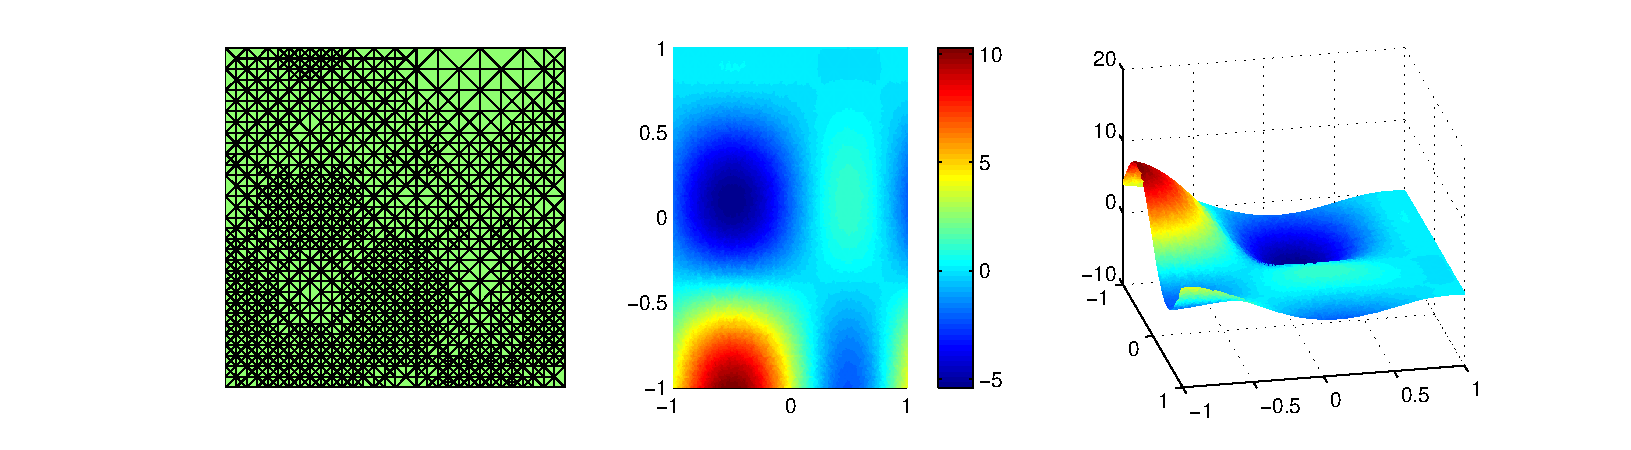
\includegraphics[width=12cm,height=15cm]{figures/iter_20.eps}
%\end{newappendix}
%
%\begin{newappendix}{Second}{2}
%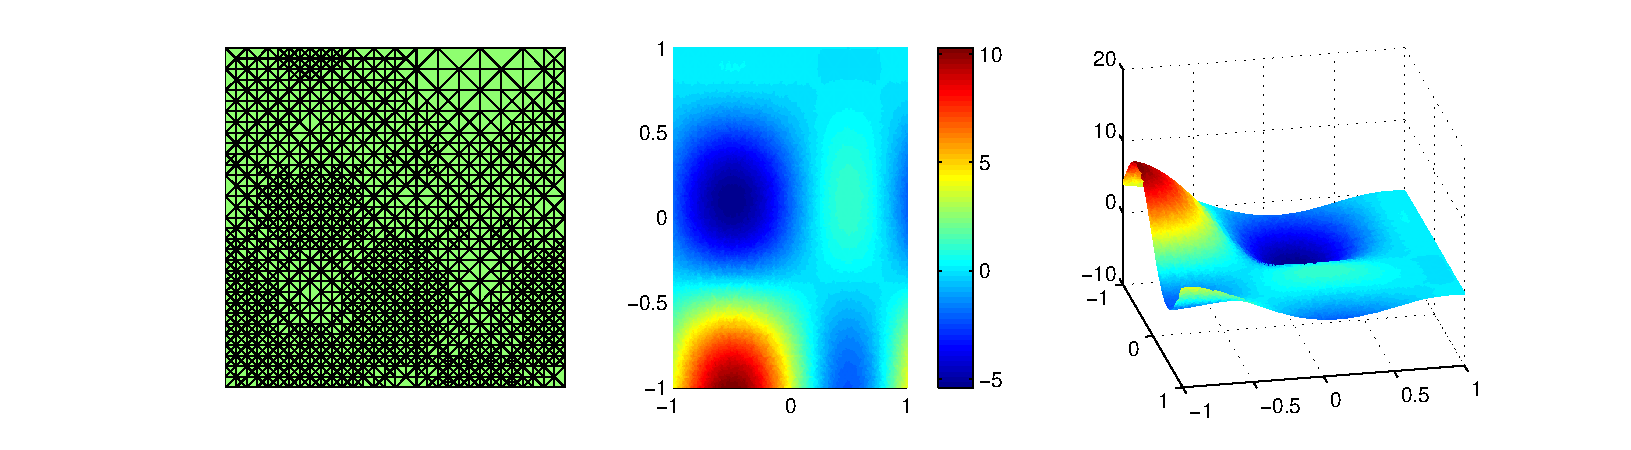
\includegraphics[width=12cm,height=15cm]{figures/iter_20.eps}
%\end{newappendix}
%%%%%%%%%%%%%%%%%%%%%%%%%%%%%%%%%%%%%%%%%%%%%%%%%%%%%%%%%%%%%%%%%%%%%%%%%%%%%%%%%%%%%%%%%%%%%%%%%%%%%%%
\end{document}
